%% Road to VPhO 2023 Template

\documentclass[12pt]{article}
% \usepackage[english]{babel}
\usepackage[utf8]{vietnam}
\usepackage[T5]{fontenc}
\usepackage[top=2cm, bottom=2cm, left=2cm,right=2cm]{geometry}
%% Margin %%

%%%%%%%%%% Figure %%%%%%%%%%%%%
\usepackage[pdftex]{graphicx}
\usepackage{subcaption}
\usepackage{wrapfig}

\usepackage[dvipsnames]{xcolor}
\usepackage[pdftex]{graphicx}
\usepackage{wrapfig}
\usepackage{tcolorbox}
\usepackage{mathtools}
\usepackage{amsmath}
\usepackage{amssymb}
\usepackage{eqnarray}
\usepackage{siunitx}
\usepackage{array, lipsum, bibentry,fancyhdr}
\usepackage{hyperref}
\usepackage{natbib}
\setlength{\parindent}{0pt}
\usepackage{enumitem}
\usepackage[noframe]{showframe}
\usepackage{framed}
\usepackage{titling}
\usepackage{float}
\usepackage{multicol}
\usepackage{url}
\usepackage{authblk}
\usepackage{sectsty}
\usepackage{eqparbox}
\usepackage{dsfont}


%%%%%%%%%% Pictures drawing %%%%%%%%%%%%%

\usepackage{pgfplots} %%%%%% Regression %%%%
\pgfplotsset{compat = newest}
\usepackage{pgfplotstable}
\usepackage{tikz}
\usepackage{tikz-3dplot} %%%%%% Draw %%%%%%
\usepackage{tikz,tkz-euclide}
\usetikzlibrary{arrows,calc,patterns}
\usetikzlibrary{quotes,angles}
\usetikzlibrary{shapes.geometric}
\usepackage{circuitikz} %%%%% Circuit %%%%
\usetikzlibrary{decorations.pathmorphing,patterns}

\setlength{\unitlength}{1cm}

%%%%%%%%%% Hyperlink %%%%%%%%%%%%%

\hypersetup{
	colorlinks=true,
	linkcolor=black,
	filecolor=mangeta,      
	urlcolor=blue,
	pdftitle={Overleaf Example},
	pdfpagemode=FullScreen,
}

%%%%%%%%%% Header & Footer %%%%%%%%%%%%%

\setlength{\headheight}{10mm}
\RequirePackage{fancyhdr}  % Needed to define custom headers/footers
\RequirePackage{lastpage}  % Number of pages in the document
\pagestyle{fancy}          % Enables the custom headers/footers
% Headers
\lhead{\includegraphics[width=.8in]{xPhO.png}}%
\chead{}%
\rhead{\small\sffamily\bfseries{Đề bài lội tới xPhO 2025} --- \thepage/\pageref{LastPage}}
% Footers
\lfoot{}%
\cfoot{}%
\rfoot{}%
\renewcommand{\headrulewidth}{1pt}% % header rule
\renewcommand{\footrulewidth}{1pt}% % footer rule

% \pagestyle{fancy}
% 	\fancyhead[L]{\empty}
% 	\fancyhead[R]{\empty}
% 	\fancyhead[C]{\empty}
% 	\fancyfoot[C]{\empty}
% 	\fancyfoot[L]{\empty}
% 	\renewcommand{\headrulewidth}{0pt}
% 	\fancyfoot[C]{\normalcolor{\thepage/\pageref{LastPage}}}
% 	\setcounter{page}{1}

%%%%%%%%%% Color setup %%%%%%%%%%%%%

\RequirePackage{xcolor}
\definecolor{wsdred}{HTML}{8E1728}
\definecolor{wsdgrey}{HTML}{75787B}
\renewcommand{\normalcolor}{\color{wsdred}}
\colorlet{ColorOr}{white}

\begin{document}

%% Title %%
{\fontsize{50}{24}\fontfamily{phv}\fontseries{b}
\LARGE \normalcolor{ \textbf{Đề bài lội tới xPhO 2025} } }

\textcolor{blue}{\textbf{\textit{Câu lạc bộ vật lý xPhO}}}

\textit{Phiên bản ngày: \today}
%%%%
\vspace{5mm}

{\normalcolor\textbf{CÂU 1.}}\vspace{1.5mm}

\setcounter{equation}{0}
\textbf{Lắc đều trước khi uống}

\textbf{1.} Một cốc nước hình trụ bán kính \(R\), chứa hai loại chất lỏng có khối lượng riêng \(\rho_1\) và \(\rho_2\). Ở trạng thái tĩnh ban đầu, chất lỏng \(\rho_1\) nằm dưới và có độ cao \(h_1\), chất lỏng \(\rho_2\) nằm trên cao \(h_2\). Quay cốc nước này quanh trục đối xứng với vận tốc \(\omega\). Xét trạng thái cốc nước quay ổn định và các chất lỏng không trộn vào nhau. Gia tốc trọng trường là \(g\).

\textbf{a.} Chứng minh rằng mặt ngăn cách giữa hai lớp chất lỏng là mặt Paraboloid.

\textbf{b.} Với các vận tốc góc quay \(\omega\) khác nhau, hình dạng của các mặt nước cũng thay đổi. Hình \ref{fig:Rotating_cup} là hình ảnh phân bố nước trong cốc đối với các trường hợp vận tốc góc \(\omega\) tăng dần từ trái sang phải. Vận tốc góc \(\omega_1\), \(\omega_2\), \(\omega_3\) lần lượt là các vận tốc góc ứng với 3 trường hợp hình \ref{fig:Rotating_cup}b, hình \ref{fig:Rotating_cup}c và \ref{fig:Rotating_cup}d. Xác định điều kiện trị của \(\omega_1\), \(\omega_2\) và \(\omega_3\) theo \(R\), \(h_1\), \(h_2\) và \(g\).

\textbf{c.} Xác định độ cao \(z_{max}\) so với đáy của điểm cao nhất trên mặt nước trong trường hợp hình \ref{fig:Rotating_cup}d.

\begin{figure}[!h]
    \centering
    \includegraphics[width=0.9\linewidth]{Problem_1/Figs_P1/Rotating_cup.pdf}
    \caption{Các trường hợp mặt nước khi tăng dần tốc độ quay của cốc.}
    \label{fig:Rotating_cup}
\end{figure}

\textbf{2.} Thay vì hai chất lỏng ở phần 1, ta đổ vào cốc nước một chất lỏng với độ cao ban đầu \(h_0\). Sau một thời gian, các phần cặn của chất lỏng này lắng xuống đáy cốc, tạo thành sự phân bố khối lượng riêng chất lỏng dạng \(\rho=\rho_0 ( 1 - \alpha z)\). Quay chậm cốc nước này quanh trục đối xứng với vận tốc \(\omega\). Xác định phân bố khối lượng riêng của chất lỏng \(\rho (r, z)\). Xem rằng khi quay cốc, khối lượng riêng của từng phần tử nước không bị thay đổi.

\textit{Lưu ý: Trong bài toán này, ta chọn gốc tính áp suất tương đối bằng không tại một điểm trong không khí.}
\setcounter{equation}{0}
% \begin{center}
%     \normalcolor{\textbf{Bài giải}}
% \end{center}
% \textbf{1.} 

\textbf{1a.} Xét một phần tử chất lỏng tại mặt phân cách giữa hai môi trường. Để phần tử chất lỏng này cân bằng, các lực tiếp tuyến tác dụng vào phần tử từ các phía phải bằng nhau, tức áp suất trên toàn bộ mặt ngăn cách giữa hai môi trường bằng nhau. Như vậy, mặt phân cách giữa hai môi trường phải là một "mặt đẳng áp"\footnote{Các lời giải thích khác xuất phát từ \(\nabla \times \rho \mathbf{g'} = 0\) dẫn tới hàm áp suất \(p\) là hàm thế vị có ý nghĩa tương tự.}.

Phân bố áp suất chất lỏng ở trong hai miền chất lỏng \(\rho_1\) và \(\rho_2\) lần lượt tuân theo hai biểu thức:
\begin{equation}
    p_1(r,z) = p_{10} - \rho_1 g z + \rho_1 \dfrac{\omega^2r^2}{2g},
\end{equation}
và
\begin{equation}
    p_2(r,z) = p_{20} - \rho_2 g z + \rho_2 \dfrac{\omega^2r^2}{2g},
\end{equation}
trong đó, \(p_{10}\) và \(p_{20}\) là hai hằng số thể hiện gốc tính áp suất tương đối.

Tại mặt ngăn cách giữa hai môi trường thì \(p_1(r,z) = p_2(r,z)\), tức là mặt ngăn cách này có phương trình mô tả bề mặt
\begin{equation}
    z = \dfrac{\omega^2 r^2}{2g} + \dfrac{p_{20} - p_{10}}{g\left( \rho_2 - \rho_1 \right)}.
\end{equation}

Như vậy, mặt ngăn cách giữa hai môi trường là một mặt Paraboloid.

\textbf{1b.}

\textit{\textbf{Lưu ý:} Dựa vào một phép tích phân cơ bản, ta có thể chứng minh rằng mặt Paraboloid bên trên chia hình trụ bản kính \(r\) độ cao \(z\) thành hai khối có thể tích bằng nhau và bằng một nửa thế tích hình trụ.}

Trường hợp mặt nước phân bổ như hình \ref{fig:Rotating_cup}b xảy ra khi thể tích chất lỏng \(\rho_1\) lớn hơn nửa dưới hình trụ bán kính R được chia bởi Paraboloid, tức là
\begin{equation}
    \pi R^2 h_1 \ge \dfrac{1}{2} \pi R^2 \dfrac{\omega_1^2 R^2}{2g} \Rightarrow \omega_1 \le 2 \dfrac{ \sqrt{g h_1}}{R}.
\end{equation}

Trường hợp \ref{fig:Rotating_cup}d xảy ra khi tổng thể tích hai chất lỏng nhỏ hơn nửa dưới hình trụ bán kính \(R\) được chia bởi Paraboloid, tức là
\begin{equation}
    \pi R^2 \left( h_1 + h_2 \right) \le \dfrac{1}{2} \pi R^2 \dfrac{\omega_3^2 R^2}{2g} \Rightarrow \omega_3 \ge 2 \dfrac{ \sqrt{g \left( h_1 + h_2 \right) }}{R}.
\end{equation}

Trường hợp còn lại như hình \ref{fig:Rotating_cup}c xảy ra khi
\begin{equation}
    2 \dfrac{ \sqrt{g h_1 }}{R} \le \omega_2 \le 2 \dfrac{ \sqrt{g \left( h_1 + h_2 \right)}}{R}
\end{equation}

\textbf{1c.}

Gọi bán kính của vùng đáy bình không chưa chất lỏng ở hình \ref{fig:Rotating_cup}d là \(R_0\).

\begin{figure}[!h]
    \centering
    \includegraphics[width=0.9\linewidth]{Problem_1/Figs_P1/Boolean_water.pdf}
    \caption{Cách tính thể tích phần chất lưu hình \ref{fig:Rotating_cup}d.}
    \label{fig:Boolean_water}
\end{figure}

Thể tích tổng lượng chất lỏng lúc sau (được tính theo hình \ref{fig:Boolean_water}) bằng với thể tích chất lưu lúc đầu nên
\begin{equation}
    \dfrac{1}{2} \pi R^2 \dfrac{\omega^2 R^2}{2g} + \dfrac{1}{2} \pi R_0^2 \dfrac{\omega^2 R_0^2}{2g} - \pi R^2 \dfrac{\omega^2 R_0^2}{2g} = \pi R^2 \left( h_1 + h_2 \right) \Rightarrow R_0 = \sqrt{R^2 - 2 R \sqrt{\dfrac{g\left( h_1 + h_2 \right)}{\omega^2}}}.
\end{equation}

Độ cao của mực nước là
\begin{equation}
    z_{max} = \dfrac{\omega^2 R^2}{2g} - \dfrac{\omega^2 R_0^2}{2g} = R \sqrt{\dfrac{\omega^2 \left( h_1 + h_2 \right)}{g}.}
\end{equation}

\textbf{2.}

Phân bố khối lượng riêng được chia thành 2 dạng hàm khác nhau (hình \ref{fig:Density_distribution}a). Với miền giá trị \(z - \dfrac{\omega^2 r^2}{2g} \ge 0\), các lớp nước có cùng độ dày, đồng dạng và tịnh tiến theo phương thẳng đứng. Mặt khác, trong miền giá trị \(z - \dfrac{\omega^2 r^2}{2g} \le 0\), các lớp cùng khối lượng riêng không còn có độ dày bằng nhau, yêu cầu các tính toán cẩn thận và phức tạp hơn.

\begin{figure}[!h]
    \centering
    \includegraphics[width=0.9\linewidth]{Problem_1/Figs_P1/Density_distribution.pdf}
    \caption{\textbf{(a)} Phân bố khối lượng riêng trong cốc nước, màu hồng nhạt ở giữa ứng với lượng chất lỏng có khối lượng riêng nằm trong dải giá trị \(\rho_0 \left( 1 - \alpha \dfrac{\omega^2 R^2}{4g} \right)\) đến \(\rho(z,R)\); \textbf{(b)} Cách tính thể tích lượng chất lỏng có khối lượng riêng nằm trong dải giá trị \(\rho_0 \left( 1 - \alpha \dfrac{\omega^2 R^2}{4g} \right)\) đến \(\rho(z,R)\).}
    \label{fig:Density_distribution}
\end{figure}

Với \(z - \dfrac{\omega^2 r^2}{2g} \ge 0\)

\begin{equation}
    \rho = \rho_0 \left[ 1 + \alpha \left( - z + \dfrac{\omega^2 r^2}{2g} - \dfrac{\omega^2 R^2}{4g} \right) \right]
\end{equation}


Với \(z - \dfrac{\omega^2 r^2}{2g} \le 0\)

Theo hình \ref{fig:Density_distribution}b, thể tích lượng nước có khối lượng riêng nằm trong dải giá trị từ \(\rho_0 \left( 1 - \alpha \dfrac{\omega^2 R^2}{4g} \right)\) đến \(\rho(R, z)\) là
\begin{equation}
    \dfrac{\rho(R, z) - \rho_0 \left( 1 - \alpha \dfrac{\omega^2 R^2}{4g} \right)}{\rho_0 \alpha} \pi R^2  = \left( \dfrac{\omega^2 R^2}{2g} - z \right) \pi R^2 - \dfrac{1}{2} \left( \dfrac{\omega^2 R^2}{2g} - z \right) \pi \left( R^2 - \dfrac{2gz}{\omega^2} \right).
\end{equation}

Giải phương trình trên, ta được
\begin{equation}
    \rho (R, z) = \rho_0 \left( 1 - \alpha \dfrac{g z^2}{\omega^2 R^2} \right).
\end{equation}

Theo phương trình điều kiện mặt đẳng thế

\begin{equation}
    \rho (r, z) = \rho \left( R, z + \dfrac{\omega^2 (R^2 - r^2)}{2g} \right) = \rho_0 \left[ 1 - \alpha \dfrac{g}{\omega^2 R^2} \left( z + \dfrac{\omega^2R^2}{2 g} - \dfrac{\omega^2 r^2}{2g} \right)^2 \right].
\end{equation}

Vậy
\begin{equation}
    \rho (r,z) = \left\{
    \begin{array}{cll}
        \rho_0 \left[ 1 - \alpha \left( z - \dfrac{\omega^2 r^2}{2g} + \dfrac{\omega^2 R^2}{4g} \right) \right], & \text{nếu} \ z - \dfrac{\omega^2 r^2}{2g} \ge 0, \\
        \rho_0 \left[ 1 - \alpha \dfrac{g}{\omega^2 R^2} \left( z - \dfrac{\omega^2 r^2}{2g} + \dfrac{\omega^2R^2}{2 g} \right)^2 \right], & \text{nếu} \ z - \dfrac{\omega^2 r^2}{2g} \le 0.
    \end{array}
    \right.
\end{equation}
\begin{flushright}
    (Biên soạn bởi Log).
\end{flushright}
\newpage
{\normalcolor \textbf{CÂU 2.}}\vspace{1.5mm}

\setcounter{equation}{0}

\textbf{1. Định luật Richardson cho kim loại}
\begin{figure}[!htb]
    \centering
    \includegraphics[width=0.6\linewidth]{Problem_2/Figs_P2/Kim loại_1.pdf}
    \caption{(A) Hộp \(L \times L \times L\); (B) Không gian \((k_x,k_y)\); (C) Hệ tuần hoàn}
    \label{fig:kim loại}
\end{figure}


\begin{enumerate}[label = \textbf{\roman*.}]
    \item Cho \(\psi(\mathbf{k},\mathbf{r})\) là hàm sóng của một electron bị giam trong một hộp có thể tích \(V = L \times L \times L\). Ứng với một giá trị \(\mathbf{k}  = (k_x,k_y,k_z)\) là một \textit{state -  trạng thái} của electron đó. Vector \(\mathbf{r}\) có gốc là tâm của hình hộp. 
    \begin{equation}
        \psi(\mathbf{k}, \mathbf{r}) = \frac{1}{\sqrt{L^3}} e^{i \mathbf{k} . \mathbf{r}} .
        \label{eq:P2_1}
    \end{equation}
    Ta lập được một không gian của vector \(\mathbf{k}\). Trong không gian \(\mathbf{k}\), những trạng thái (stated) được biểu diễn như những điểm có toạ độ \((k_x,k_y,k_z)\). Ở hình \ref{fig:kim loại}b ta mô tả cho trường hợp 2 chiều, ta thấy rằng các trạng thái là những điểm rời rạc. 
    \begin{enumerate}[label = \textbf{\alph*)}]
        \item Chứng minh điều kiện của \(\mathbf{k}\) để hệ vật lý là hệ tuần hoàn thoả các phương trình
        \begin{equation}
            k_x = \frac{2\pi n_x}{L}; \  k_y = \frac{2\pi n_y}{L}; \ k_x = \frac{2\pi n_x}{L}.
        \end{equation}
        Với \((n_x,n_y,n_z)\) là các số nguyên thuộc \(\mathds{Z}\). Hệ tuần hoàn có tính lặp lại theo chu kỳ. Khi đấy ta coi có nhiều hộp xếp kế bên nhau (Hình \ref{fig:kim loại}c). Ta gọi mỗi một hộp là một ô cơ sở.
        \item Trong không gian \(\mathbf{k}\), khoảng cách giữa các điểm trạng thái liền kề nhau? Xét một thể tích \( \mathrm{d} V_{\mathbf{k}}\) theo toạ độ cầu, tìm vi phân \(\mathrm{d} N\) trạng thái mà \(\mathrm{d} V_{\mathbf{k}}\) bao lấy. Biết rằng \(\mathrm{d} N\) có thể viết dưới dạng sau, với \(g(E)\) được gọi là mật độ trạng thái. Tìm \(g(E)\).
        \begin{equation}
            \mathrm{d} N = g(E) \mathrm{d} E = g(k) \mathrm{d} k = g(v) \mathrm{d} v.
        \end{equation}
        
        *Biết electron có spin up và spin down, nghĩa là ở cùng một mức năng lượng có thể tồn tại nhiều nhất 2 electron có spin ngược nhau.
        
        \item Tìm hàm mật độ trạng thái \(g(k), \ g(v)\) với các biến \(k\) và tốc độ \(v\).
        \vspace{2mm}

        \textit{*Công thức liên hệ giữa năng lượng \(E\) và \(k\) là \(\displaystyle E = \frac{\hbar^2 k^2}{2m}\).}
    \end{enumerate}
    \item Biết electron tuân theo phân bố Fermi-Dirac. Phân bố Fermi-Dirac là trung bình số hạt có năng lượng \(E\) trên tổng \(dN\) hạt.
    \begin{equation}
        f_{FD}(E) = \frac{1}{1 + \exp{\displaystyle \left[\frac{E - E_F}{kT} \right]}}.
        \label{eq:P2_2}
    \end{equation}
    \begin{enumerate}[label = \textbf{\alph*)}]
        \item Tìm mật độ số hạt  \(\mathrm{d}n(E) \ \big[\text{Hạt}/ L^3 \big]\) có năng lượng trong khoảng \(\Big[E, E + dE\Big]\).
        \item Nếu electron có mức vận tốc đủ lớn để thoát khỏi thế năng giam cầm \(U\) thì sẽ tạo một mật độ dòng \(j_x\) theo phương \(Ox\), tính mật độ \(j_x\). Biết rằng, để electron thoát khỏi kim loại thì \(E \gg E_F\). 
    \end{enumerate}
\end{enumerate}
\textbf{2. Graphene single-layer}
\vspace{2mm}

\begin{figure}[!htb]
    \centering
    \includegraphics[width=0.75\linewidth]{Problem_2/Figs_P2/Graphene.pdf}
    \caption{(A) GSL; (B) electron trong GSL.}
    \label{fig:graphene}
\end{figure}
\newpage
Vật liệu Graphene single-layer (GSL) là một vật liệu 2D (kích thước \(L \times L\)), các electron chủ yếu chuyển động song song với bề mặt của GSL. Một tính chất đặc biệt của GSL là electron chuyển động song song sẽ di chuyển với vận tốc đều \(\mathbf{v_F}\). Và năng lượng cho chuyển động song song của chúng là
\begin{equation}
    E_p = \hbar v_F |\mathbf{k}|. 
\end{equation}
Ở phương vuông góc, GSL coi như vẫn có một độ dày. Electron di chuyển theo phương vuông góc sẽ coi như bị nhốt trong hố thế, với độ cao bằng với thế năng thoát của GSL. 
\begin{enumerate}[label = \textbf{\roman*.}]
    \item Tìm mật độ trạng thái \(g(E_p)\) của các electron có mức năng lượng trong khoảng \(\Big[E_p, E_p + \mathrm{d} E_p \Big]\).
    \item Từ liên hệ \(E_p + E_x = E\), tìm mật độ hạt \(\mathrm{d} n(E_x)\) của các electron có mức năng lượng trong khoảng \(\Big[E_x, E_x + \mathrm{d} E_x \Big]\). Từ đó tính ra được mật độ dòng \(j_x\).
    \vspace{2mm}

    \textit{*Gợi ý: Tính mật độ hạt \(\mathrm{d} n(E_p, E_x)\) cho các các hạt có đồng thời hai mức năng lượng trong khoảng \(\Big[E_p, E_p + \mathrm{d}E_p \Big]\) và \(\Big[E_x, E_x + \mathrm{d} E_x \Big]\) trước.}
\end{enumerate}



\setcounter{equation}{0}
% \begin{center}
%     \normalcolor{\textbf{Bài giải}}
% \end{center}
% \textbf{1.}
\begin{enumerate}[label = \textbf{\roman*.}]
    \item \textbf{a)} 
    
    Ta nhận xét rằng nếu \(\psi(\mathbf{r})\) là một hàm tuần hoàn, thì nó thoả
    \begin{equation}
        \psi(\mathbf{r}) = \psi(\mathbf{r} + \mathbf{U}). 
    \end{equation}
    
    Vector \(\mathbf{U}\) là chu kỳ của sự tuần hoàn này. Trước tiên ta xét trường hợp tuần hoàn theo một trục, ở đây ta chọn trục Ox. 

    \begin{figure}[!htb]
        \centering
        \includegraphics[width=0.9\linewidth]{Problem_2/Figs_P2/sol_Periodic.pdf}
        \caption{Hệ tuần hoàn}
        \label{fig:sol_periodic}
    \end{figure}
    
    Ta lúc này viết được
    \begin{equation}
    \notag
        \psi(x) = \psi(x+L) = \psi(x+2L) = ... = \psi(x+nL).
    \end{equation}
    Một cách tổng quát với trường hợp 3 chiều, ta lúc này viết được vector \(\mathbf{U}\)
    \begin{equation}
        \mathbf{U} = 
        \left(
        \begin{matrix}
            n_x L \\
            n_y L \\
            n_z L
        \end{matrix}
        \right) = 
        \left(
        \begin{matrix}
            n_x  \\
            n_y  \\
            n_z 
        \end{matrix}
        \right) L.
    \end{equation}
    Ta xét tính tuần hoàn của hệ hộp \(L \times L \times L\), tại điểm \((-\frac{L}{2},0,0)\) và điểm \((\frac{L}{2},0,0)\).
    \begin{equation}
        \exp{\left(\displaystyle -i k_x \frac{L}{2}\right)} = \exp{\left(\displaystyle i k_x \frac{L}{2}\right)}.
    \end{equation}
    Có thể sử dụng hệ thức Euler để tiếp tục giải quyết, ta thu được
    \begin{equation}
        k_x = \frac{2\pi n_x}{L}.
    \end{equation}
    Ta làm tương tự với các trục khác.
    \vspace{2mm}

    \textbf{b)}
    \vspace{2mm}

    Khoảng cách giữa hai trạng thái bất kì đơn giản chỉ cần xét 
    \begin{equation*}
        k_x(n_x) - k_x(m_x) = \frac{2\pi (n_x - m_x)}{L}. 
    \end{equation*}
    Vậy khoảng cách giữa hai trạng thái liền kề là
    \begin{equation}
        d = \frac{2\pi}{L}.
    \end{equation}

    %hình 2
    \begin{figure}[!htb]
        \centering
        \includegraphics[width=0.7\linewidth]{Problem_2/Figs_P2/sol_unitcell.pdf}
        \caption{Chọn ô cơ sở cho 1 trạng thái.}
        \label{fig:sol_unitcell}
    \end{figure}

    Trong không gian vector \(\mathbf{k}\), ta tìm thể tích \(V_1\) để luôn luôn chứa đúng 1. Ta có hai cách để tìm, như hình \ref{fig:sol_unitcell}. Trước tiên, ta tính toán cho trường hợp 2 chiều, trường hợp 3 chiều hoàn toàn tương tự. Với trường hợp 2 chiều, ta sẽ đi tìm diện tích \(S_1\) thay vì thể tích.
    \begin{equation}
        S_1 = \left( \frac{2 \pi}{L} \right)^2 = \frac{\text{Diện tích}}{\text{Số trạng thái}}.
    \end{equation}
    %hình 3
    \begin{figure}[!htb]
        \centering
        \includegraphics[width=0.5\linewidth]{Problem_2/Figs_P2/sol_densityofstate.pdf}
        \caption{\(\mathrm{d}S_\mathbf{k} \) bao lấy những trạng thái. }
        \label{fig:sol_densityofstate}
    \end{figure}
    Nếu ta chọn một diện tích \(\mathrm{d}S_{\mathbf{k}} = k \mathrm{d}k \mathrm{d}\theta \), ta sẽ tính được số trạng thái mà \(\mathrm{d}S\) bao lấy.
    \begin{equation}
    \notag
        \mathrm{d}N = 2 \frac{\mathrm{d}S_{\mathbf{k}}}{S_1} = 2  \left(\frac{L}{2 \pi}\right)^2 k \mathrm{d}k \mathrm{d}\theta.
    \end{equation}
    Số "\(2\)" ở đây ý nói "với một mức năng lượng, tồn tại hai electron". Như vậy, ta tính được thể tích chứa đúng 1 trạng thái và số trạng thái mà vi phân thể tích \(\mathrm{d}V_{\mathbf{k}}\) chứa.
    \begin{equation}
        V_1 = \left( \frac{2 \pi}{L} \right)^3 \ \ \text{và} \ \ \mathrm{d}N = 2\left(\frac{L}{2 \pi}\right)^3 (4\pi k^2 \mathrm{d}k) = \frac{L^3}{\pi^2} (k^2 \mathrm{d}k).
    \end{equation}
    Hệ thức liên hệ giữa số \(k\) và năng lượng là 
    \begin{equation}
        E = \frac{\hbar^2 k^2}{2m}.
    \end{equation}
    Thay vì tính theo biến vector sóng \(k\) ta đổi sang biến \(E\)
    \begin{equation}
    \notag
        \mathrm{d}N =  \frac{L^3}{\pi^2} k^2 \mathrm{d}k = \frac{L^3}{\pi^2} \left(\frac{2m}{\hbar^2} \right)^{3/2} \sqrt{E} \mathrm{d}E.
    \end{equation}
    Vậy hàm mật độ trạng thái là 
    \begin{equation}
        g(E) =  \frac{L^3}{\pi^2} \left(\frac{\sqrt{2} m^{3/2}}{\hbar^2} \right) \sqrt{E}.
    \end{equation}
    \textbf{c)}
    \vspace{2mm}

    Ta ngay lập tức suy ra được \(g(k)\)
    \begin{equation}
        g(k) = \frac{L^3}{\pi^2} k^2.
    \end{equation}
    Ta có hệ thức động năng
    \begin{equation}
        E = \frac12 m v^2.
    \end{equation}
    Làm tương tự ta có 
    \begin{equation}
        g(v) =  \left(\frac{mL}{\hbar}\right)^3 \frac{v^2}{\pi^2}.
    \end{equation}
    \item \textbf{a)}
    \vspace{2mm}

    Với mức năng lượng \(\Big[E, E + \mathrm{d}E \Big]\), ta sẽ đếm được \(\mathrm{d}N\) hạt (như ở phần \textbf{i.} chúng ta vừa làm). Nhưng thực tế, chỉ có một phần trong \(\mathrm{d}N\) hạt có mức năng lượng \(\Big[E, E + \mathrm{d}E \Big]\). Lý do thực sự là do mật độ của hạt đủ lớn hoặc nhiệt độ hạt đủ lớn. Lúc này các quy luật thống kê sẽ bị thêm chi phối của các quy tắc lượng tử.
    \vspace{2mm}

    Các hạt electron là hạt Fermion (tuân theo phân bố Fermi-Dirac) sẽ tồn tại dựa trên nguyên lý loại trừ Pauli \textit{"Với một mức năng lượng, chỉ cho phép tồn tại nhiều nhất 2 hạt"}. Có thêm một phân bố lượng tử nữa là của hạt Boson (tuân theo phân bố Bose-Einstein), các hạt Boson có thể \textit{tồn tại vô hạn} các hạt ở cùng một mức năng lượng. Ví dụ của hạt Boson là photon ánh sáng.
    \vspace{2mm}

    Quay lại với bài toán, ta có thể tính được mật độ số hạt có mức năng lượng \(\Big[E, E + \mathrm{d}E \Big]\) như sau
    \begin{equation}
        \mathrm{d} n(E) = \frac{f_{FD} \  \mathrm{d}N}{L^3} = \frac{\displaystyle \frac{1}{\pi^2} \frac{\sqrt{2}m^{3/2}}{\hbar^2}}{1 + \exp{\displaystyle \left[\frac{E - E_F}{k_bT} \right]}}  \sqrt{E} \mathrm{d}E
    \end{equation}
    \textbf{b)}
    \vspace{2mm}

    Mật độ dòng được tính như sau, ta vẫn có thể dùng \(n(k)\) hoặc \(n(E)\) tuỳ theo sở thích.
    \begin{equation}
        j_x =  \int e v_x \mathrm{d} n(v) .
    \end{equation}
    Lưu ý, ta có thể sử dụng xấp xỉ \(E \ll E_F\)
    \begin{equation}
        f_{FD} = \frac{1}{1 + \exp{\displaystyle \left[\frac{E - E_F}{k_bT}  \right]}} \simeq \exp{\displaystyle \left[-\frac{E - E_F}{k_bT}  \right]}.
    \end{equation}
    Ta có thể tính được \(n(v)\) 
    \begin{equation}
        \mathrm{d} n(v) =  \frac{f_{FD} \ dN}{L^3} = \left(\frac{m}{\hbar}\right)^3 \exp{\displaystyle \left[-\frac{\frac12 m v^2 - E_F}{k_bT}  \right]} \frac{1}{\pi^2} v^2 \mathrm{d}v. 
    \end{equation}
    Từ đây lắp vô công thức mật độ dòng \(j_x\)
    \begin{equation}
        \notag
        j_x = \frac{e}{\pi^2} \left(\frac{m}{\hbar}\right)^3 \int v_x  \exp{\displaystyle \left[-\frac{\frac12 m v^2 - E_F}{k_bT}  \right]}  v^2 \mathrm{d}v
    \end{equation}
    Để thuận tiện cho việc tích phân, ta đổi hệ toạ độ cầu sang hệ toạ độ Descartes. 
    \begin{equation*}
        4 \pi v^2 \mathrm{d}v = \mathrm{d} v_x \mathrm{d} v_y \mathrm{d} v_z.
    \end{equation*}
    Vậy, lúc này ta có thể tách \(j_x\) thành 3 tích phân
    \begin{equation}
    \begin{split}
        j_x = \frac{e}{4\pi^3} \left(\frac{m}{\hbar}\right)^3  \exp\left[\frac{E_F}{k_bT}\right] 
        \int_{v_0}^{\infty} v_x  &\exp{\displaystyle \left[-\frac{ m v_x^2 }{2k_bT}  \right]} \mathrm{d} v_x \\ \\ &\int_{-\infty}^{\infty }  \exp{\displaystyle \left[-\frac{ m v_y^2 }{2k_bT}  \right]} \mathrm{d} v_y \int_{-\infty}^{\infty }   \exp{\displaystyle \left[-\frac{ m v_z^2 }{2k_bT}  \right]} \mathrm{d} v_z.
    \end{split}
    \end{equation}
    Ở đây, \(v_0\) là vận tốc tối thiểu để vật có thể thẳng được thế năng giảm cầm của mạng tinh thể; \(A\) là công thoát tương ứng.
    \begin{equation}
        \begin{split}
            I_1 &= \int_{v_0}^{\infty} v_x  \exp{\displaystyle \left[-\frac{ m v_x^2 }{2k_bT}  \right]} \mathrm{d} v_x =  \frac{k_bT}{m} \exp \left[-\frac{m v_0^2}{2k_bT}\right] = \frac{k_bT}{m} \exp \left[-\frac{A}{k_bT}\right] \\
            I_2 &= \int_{-\infty}^{\infty }  \exp{\displaystyle \left[-\frac{ m v_y^2 }{2k_bT}  \right]} \mathrm{d} v_y = \sqrt{\frac{2 \pi k_bT}{m}}\\
            I_3 &= \int_{-\infty}^{\infty }   \exp{\displaystyle \left[-\frac{ m v_z^2 }{2k_bT}  \right]} \mathrm{d} v_z = \sqrt{\frac{2 \pi k_bT}{m}}.
        \end{split}
    \end{equation}
    Vậy, ta tính được mật độ dòng là 
    \begin{equation}
        j_x = \frac{emk^2T^2}{2 \pi^2 \hbar^3} \exp\left[-\frac{A-E_F}{k_bT}\right].
    \end{equation}
\end{enumerate}
\textbf{2.}
\begin{enumerate}[label = \textbf{\roman*.}]
    \item Với các hạt chuyển động song song với tấm vật liệu, lúc này chúng chỉ có 2 thành phần vận tốc. Tương ứng với không gian \(\mathbf{k_p}\) là một mặt phẳng (giống hệt hình \ref{fig:kim loại}b). Ta tính được mật độ trạng thái \(g(k_p)\)
    \begin{equation}
    \notag
        g(k_p) = \frac{L^2}{\pi}k_p \mathrm{d}k_p
    \end{equation}
    Từ đây tìm được mật độ trạng thái \(g(E_p)\)
    \begin{equation}
        g(E_p) =  \frac{L^2}{\pi} \frac{E_p}{(\hbar v_F)^2} \mathrm{d} E_p.
    \end{equation}
    \item Nhưng lúc này ta chưa thể nhân thêm phân bố \(f_{FD}\) và nhận định rằng nó là \(n(E_p)\) được. Lưu ý rằng \(f_{FD}\) chỉ biểu diễn cho hạt có mức năng lượng \(E\) chứ không phải \(E_p\).
    \vspace{2mm}
    
    Những hạt có mức năng lượng \(E\) là những hạt, vừa có mức năng lượng \(E_x\) và \(E_p\). Ta vẫn đi xét một vi phân thể tích trong không gian \(\mathbf{k}\). Để thuận tiện trong việc loại trừ biến \(k_y, k_z\), ta sử dụng hệ toạ độ trụ, với chiều cao tương ứng với trục \(Ox\).
    \begin{equation}
        \mathrm{d} V_\mathbf{k} = \mathrm{d} k_x \mathrm{d} k_y \mathrm{d} k_z = 2 \pi k_p \mathrm{d}k_p \mathrm{d}k_x.
    \end{equation}
    Tổng trạng thái được thể tích \(\mathrm{d} V_\mathbf{k}\) bao lấy là
    \begin{equation}
        \mathrm{d} N = 2 \frac{2 \pi k_p \mathrm{d}k_p \mathrm{d}k_x}{\displaystyle  \left(\frac{2\pi}{L}\right)^2 }
    \end{equation}
    Ta thấy rằng, ở đây tại chỉ xét ô cơ sở 2D trên mặt phẳng \(Oyz\). Nhưng lại không hề sử dụng ô cơ sở 3D giống như phần 1. Để giải thích tại sao \(\mathrm{d}V_\mathbf{k}\) không liên quan tới sự phân bố trạng thái theo trục \(Ox\), ta giả sử lớp GSL có độ dày \(h \lll L\). Vậy khoảng cách giữa hai trạng thái liên tiếp dọc theo \(Ox\) là
    \begin{equation*}
        d_x = \frac{2\pi}{h}\ \xrightarrow{\ h \rightarrow 0 \ } \infty.
    \end{equation*}
    Như thế khoảng cách giữa 2 trạng thái trên trục \(Ox\) là rất lớn. Nên, ta không thể xấp xỉ thành từ rời rạc các trạng thái thành liên tục được. Ta hay nhận định rằng, để có thể xấp xỉ thành hệ liên tục thì độ dài vi phân \(\mathrm{d}k_x\) vẫn phải lớn hơn rất nhiều khoảng cách giữa những trạng thái (tương tự đối với lại các hệ liên tục khác như điện tích khối,...). 
    \vspace{2mm}
    
    Lúc này trong không gian \(\mathbf{k}\) ta chọn một ô \(\mathrm{d}V_\mathbf{k}\) bất kì. Theo hình \ref{fig:GSL k-space} thì \(d_x\) càng tăng, số trạng thái nằm trong \(\mathrm{d} V_\mathbf{k}\) càng giảm. Đến một giá trị nhất định, vi phân thể tích chỉ có thể bao lấy được những trạng thái thuộc mặt phẳng \(Oyz\). 
    \begin{figure}[!htb]
        \centering
        \includegraphics[width=1.07\linewidth]{Problem_2/Figs_P2/sol_GSL k-space.pdf}
        \caption{Không gian \(\mathbf{k}\) của GSL với \(d_x\) tăng dần.}
        \label{fig:GSL k-space}
    \end{figure}
    
    Từ đây, ta có thể tính được mật độ những hạt có vector sóng \(k_x, k_y, k_z\)  là 
    \begin{equation}
        \mathrm{d} n(k_x,k_p) = \frac{f_{FD} \ \mathrm{d}N}{L^2} = f_{FD} \frac{ k_p \mathrm{d}k_p \mathrm{d}k_x}{ \pi}. 
    \end{equation}
    Từ đây, ta sẽ tính toán được mật độ dòng \(j_x\)
    \begin{equation}
    \notag
    \begin{split}
        j_x &= \int e v_x \mathrm{d} n(k_x,k_p) \\
        &= \int e v_x \exp{\displaystyle \left[-\frac{E - E_F}{k_bT}  \right]} \frac{ k_p \mathrm{d}k_p \mathrm{d}k_x}{ \pi^2} \\
        &= \frac{e}{\pi} \exp{\left[\frac{E_F}{k_b T}\right]} \int v_x \mathrm{d}k_x  \int \exp{\left[-\frac{E}{k_b T}\right]} k_p \mathrm{d}k_p . \\
        &= \frac{e}{\pi} \exp{\left[\frac{E_F}{k_b T}\right]} \int_{A}^{\infty} \frac{1}{\hbar} \mathrm{d} E_x \int_{0}^{\infty}  \exp{\left[-\frac{E}{k_b T}\right]}  \frac{E_p}{(\hbar v_F)^2} \mathrm{d} E_p \\
        &= \frac{e}{\pi \hbar^3 v_F^2} \exp{\left[\frac{E_F}{k_b T}\right]} \int_{A}^{\infty} \exp{\left[-\frac{E_x}{k_b T}\right]} \mathrm{d} E_x \int_{0}^\infty \exp{\left[-\frac{E_p}{k_b T}\right]} E_p \mathrm{d}E_p.
    \end{split}
    \end{equation}
    Ta tính cách tích phân được kết quả như sau
    \begin{equation*}
        \begin{split}
        I_1 &= \int_{A}^{\infty} \exp{\left[-\frac{E_x}{k_b T}\right]} \mathrm{d} E_x = k_b T \exp{\left[-\frac{A}{k_b T}\right]}.\\
        I_2 &= \int_{0}^\infty \exp{\left[-\frac{E_p}{k_b T}\right]} E_p \mathrm{d}E_p = k_b^2 T^2.
        \end{split}
    \end{equation*}
    Vậy mật độ dòng là
    \begin{equation}
        j_x =  \frac{ek_b^3 T^3}{\pi \hbar^3 v_F^2} \exp{\left[-\frac{A-E_F}{k_b T}\right]}.
    \end{equation}
\end{enumerate}

\bibliographystyle{plain}
\begin{thebibliography}{}
\bibitem{Marjan Grilj} Marjan Grilj. "Thermionic emission". University of Ljubljana (2008).
\bibitem{Shi-Jun Liang} Shi-Jun Liang and L. K. Ang. "Electron Thermionic Emission from Graphene and a Thermionic Energy Converter." PHYSICAL REVIEW APPLIED 3, 014002 (2015).
\end{thebibliography}
\begin{flushright}
    (Biên soạn bởi Mino và Log).
\end{flushright}
\newpage
{\normalcolor\textbf{CÂU 3.}}\vspace{1.5mm}

\setcounter{equation}{0}
Phun điện (Electrospray) là hiện tượng các hạt mang điện được phóng ra từ chất lỏng phân cực hoặc dẫn điện dưới tác dụng của điện trường đủ mạnh. Thí nghiệm đầu tiên về phun điện được thực hiện vào thế kỷ 18, khi Jean-Antoine Nollet nhận thấy nước bị phun sương (tạo thành sương mù) khi chảy ra từ một bình chứa được nối với nguồn điện áp cao.

Một mao quản được chứa đầy chất lỏng dẫn điện. Khi một điện trường được áp vào đầu nơi bề mặt chất lỏng tiếp xúc với không khí, bán kính độ cong của bề mặt chất lỏng sẽ giảm xuống.

    \begin{figure}[!htb]
        \centering
        \includegraphics[width=0.4\linewidth]{Problem_3/Figs_P3/Fig1_B3.pdf}
        \caption{Mao quản đặt giữa hai cực của một nguồn điện}
        \label{fig:Electrospray}
    \end{figure}

\begin{enumerate}
    \item Nếu cường độ điện trường áp vào vẫn chưa đủ mạnh để làm cho chất lỏng phun ra thành các hạt mang điện, hãy ước tính mối quan hệ giữa bán kính cong của bề mặt chất lỏng $R_c$ và cường độ điện trường $E$ phía trên bề mặt. Giả sử hệ số sức căng bề mặt của chất lỏng là $\sigma$.
\end{enumerate}
Bây giờ ta sẽ tìm hiểu mối liên hệ giữa điện áp ngoài khi chất lỏng bắt đầu phun ra các hạt mang điện $V_{\text{start}}$ và bán kính cong $R_c$. Trên một tấm phẳng nối đất vô hạn, đặt mao quản sao cho đầu chất lỏng hướng về tấm. Thành ngoài của mao quản được duy trì ở điện áp không đổi $V$. Khoảng cách giữa đỉnh của mặt chất lỏng và tấm phẳng nối đất là $d$.

Để thuận tiện cho việc tính toán, ta xem phần ngoài của mao quản và bề mặt chất lỏng như một \textbf{mặt đôi cực đối xứng trụ} (hyperboloid có trục đối xứng), và mặt này mang một điện thế không đổi \( V \), như được minh họa ở hình bên phải. Hai tiêu điểm của mặt đôi cực này là \( \mathrm{F}\left(0;0;\dfrac{a}{2}\right) \) và \( \mathrm{F}'\left(0;0;-\dfrac{a}{2}\right) \). (Giá trị của $a$ là chưa biết).
\vspace{2mm}

Giả sử một điểm \( \mathrm{P} \) trong không gian có khoảng cách đến tiêu điểm \( \mathrm{F} \) là \( r_2 \), và đến tiêu điểm \( \mathrm{F}' \) là \( r_1 \). Khi đó, phân bố điện thế trong không gian hiển nhiên có thể được biểu diễn dưới dạng hàm của \( r_1 \) và \( r_2 \) là
$
\phi(r_1, r_2)
$.
Ta đặt các tọa độ mới như sau:
\begin{equation}
\notag
\begin{aligned}
\eta = \frac{r_1 - r_2}{a} \quad \text{và} \quad
\zeta = \frac{r_1 + r_2}{a}
\end{aligned}
\end{equation}
trong đó:
\begin{equation}
\notag
r_1=\sqrt{x^2+y^2+\left(z+\frac{a}{2}\right)^2} \quad \text { và } \quad r_2=\sqrt{x^2+y^2+\left(z-\frac{a}{2}\right)^2}
\end{equation}
Khi đó phân bố điện thế có thể được viết lại thành một hàm của \( \eta \) và \( \zeta \) là $\phi(\eta, \zeta)$.
Với cách biểu diễn theo hệ tọa độ mới này, mặt chứa phần ngoài của mao quản và bề mặt chất lỏng có thể được biểu diễn bởi $\eta = \eta_0$. Các mặt $\eta=\text{const}$ là những hyperbolic đồng tiêu (có chung cặp tiêu điểm $\mathrm{F}$, $\mathrm{F^{\prime}}$). Tương tự, các mặt $\xi=\text{const}$ cũng là những ellipsoid đồng tiêu.

\begin{figure}[!htb]
    \centering
    \includegraphics[width=1\linewidth]{Problem_3/Figs_P3/Fig2_B3.pdf}
    \caption{}
    \label{fig:Electrospray_2}
\end{figure}

\begin{enumerate}
    \item[2.] Hãy lập luận để chỉ ra rằng điện thế $\phi$ sẽ chỉ phụ thuộc độc lập vào $\eta$ (tức không phụ thuộc vào $\zeta$).
\end{enumerate}
Sau khi tính toán, người ta nhận thấy rằng hàm điện thế $\phi$ sẽ tuân theo phương trình:
\begin{equation}
\tag{i}
\frac{\partial}{\partial \eta}\left[\left(1-\eta^2\right) \frac{\partial \phi}{\partial \eta}\right]=0.
\label{i}
\end{equation}
\begin{enumerate}
    \item[3.] Từ phương trình (\ref{i}) và các điều kiện biên, hãy tìm hàm điện thế $\phi (\eta)$. Biểu diễn câu trả lời theo $\eta$, $\eta_0$ và $V$.
\end{enumerate}
Biết rằng bán kính cong của các mặt hyperbolic trong không gian phụ thuộc vào công thức sau:
\begin{equation}
\tag{ii}
\rho=a \frac{1-\eta^2}{2 \eta}\left[1+4 \frac{(x^2+y^2) / a^2}{\left(1-\eta^2\right)^2}\right].
\label{ii}
\end{equation}
\begin{enumerate}
    \item[4.] Chứng minh rằng với $R_c \ll d$, điện trường tại đỉnh của bề mặt chất lỏng là:
    \begin{equation}
    \tag{iii}
    E_{t i p}=-\frac{2 V / R_c}{\ln \left(4 d / R_c\right)}.
    \label{iii}
    \end{equation}
    Từ đó hãy tính giá trị của $V_{\text{start}}$ theo $R_c, d, \sigma$, và các hằng số vật lý liên quan. 
    
\end{enumerate}




Khi điện áp \( V \) được tăng lên đủ lớn, bán kính cong \( R_c \) tại đỉnh của bề mặt chất lỏng sẽ tiến dần về 0. Khi đó, bề mặt chất lỏng sẽ hình thành một hình nón, gọi là \textbf{nón Taylor} (\textit{Taylor cone}).
Góc đỉnh của nón Taylor được ký hiệu là \( \theta_T \).
Tại đỉnh của hình nón, hệ thống rơi vào trạng thái không ổn định, và các hạt mang điện sẽ bị phóng ra khỏi đỉnh theo hướng ra ngoài.
Tuy nhiên, ngoại trừ vùng đỉnh, bề mặt bên của nón vẫn duy trì trạng thái cân bằng giữa sức căng bề mặt và áp suất tĩnh điện.
\begin{figure}[!htb]
    \centering
    \includegraphics[width=0.5\linewidth]{Problem_3/Figs_P3/Fig3_B3.pdf}
    \caption{}
    \label{fig:Electrospray_3}
\end{figure}
\begin{enumerate}
    \item[5.] Tìm cường độ điện trường bề mặt $E_n$ như một hàm của khoảng cách $r$ từ đỉnh hình nón. Biểu diễn câu trả lời theo $\sigma, r$, và $\theta_T$.
\end{enumerate}
Cho công thức tích phân sau:
\begin{equation}
\notag
\int \frac{\mathrm{d} x}{1-x^2}=\tanh^{-1}(x)+C
\end{equation}
\setcounter{equation}{0}
% \begin{center}
%     \normalcolor{\textbf{Bài giải}}
% \end{center}
% \textbf{1.} Khi cường độ điện trường áp vào vẫn chưa đủ mạnh để làm cho chất lỏng phun ra thành
các hạt mang điện thì áp suất tĩnh điện kéo các hạt ra phải nhỏ hơn áp suất do suất căng giữ nó lại:
\begin{equation}
    \frac{1}{2} \varepsilon_0 E^2<\frac{2 \sigma}{R_c}.
    \label{eq:P3_1}
\end{equation}

\textbf{2.} Nếu điện thế \( \phi \) là một hằng số \( (V) \) trên mặt \( \eta = \eta_0 \), và bằng không trên mặt phẳng \( S \), thì toàn bộ nghiệm của \( \phi \) sẽ chỉ phụ thuộc vào \( \eta \). \vspace{1.5mm}

\textbf{3.} Từ phương trình (\ref{i}) và ý \textbf{2} ta có:
\begin{equation}
    (1- \eta ^2) \frac{\mathrm{d} \phi}{\mathrm{d} \eta}=\text{cte} \Rightarrow \mathrm{d} \phi= \text{cte}\frac{ \mathrm{d} \eta}{1- \eta ^2}.
    \label{eq:P3_2}
\end{equation}
Tích phân phương trình (\ref{eq:P3_2}) với $\phi$ chạy từ 0 đến $V$, $\eta$ chạy từ 0 đến $\eta_0$, ta tính được:
\begin{equation}
    \text{cte}=\frac{V}{\tanh^{-1}{\eta_0}}.
    \label{eq:P3_3}
\end{equation}
Khi đó dễ dàng suy ra:
\begin{equation}
    \phi=V \frac{\tanh^{-1}{\eta}}{\tanh^{-1}{\eta_0}}.
    \label{eq:P3_4}
\end{equation}

\textbf{4.} Gọi \( R^2 = x^2 + y^2 \) là bán kính trụ (cylindrical radius).  
Từ biểu thức \( \eta = \dfrac{r_1 - r_2}{a} \), ta thu được mối quan hệ giữa \( z \) và \( R \) đối với mặt hyperboloid có \( \eta \) không đổi:
\begin{equation}
a \eta = \sqrt{R^2 + \left(z + \frac{a}{2} \right)^2} - \sqrt{R^2 + \left(z - \frac{a}{2} \right)^2}.
\label{eq:P3_5}
\end{equation}
Với \( z > 0 \), phương trình (\ref{eq:P3_5}) có thể được rút gọn thành:
\begin{equation}
z = \eta \sqrt{ \frac{a^2}{4} + \frac{R^2}{1 - \eta^2} }.
\label{eq:P3_6}
\end{equation}


Khoảng cách từ đỉnh chất lỏng đến mặt phẳng nối đất là
$z(R = 0, \eta = \eta_0)=d  = \dfrac{a}{2} \eta_0$. Từ phương trình (\ref{ii}), bán kính cong $R_c$ tại đỉnh là:
\begin{equation}
    R_c=a \frac{1-\eta^2}{2 \eta}.
\end{equation}
Do đó, nếu biết \( R_c \) và \( d \), ta có thể xác định các tham số \( a \) và \( \eta_0 \):
\begin{equation}
a = 2d \sqrt{1 + \frac{R_c}{d}} \quad \text{và} \quad \eta_0 = \left(1 + \frac{R_c}{d} \right)^{-1/2}.
\end{equation}
Điện trường tại đỉnh chất lỏng là:
\begin{equation}
E_{\text{đỉnh}} = -\left. \frac{\partial \phi}{\partial z} \right|_{\text{đỉnh}} 
= -\left. \frac{\partial \phi}{\partial \eta} \cdot \frac{\partial \eta}{\partial z} \right|_{\text{đỉnh}}.
\end{equation}
Tại đỉnh ta có \( R = 0 \) và \( \eta = \eta_0 \), nên từ phương trình (\ref{eq:P3_6}):
\begin{equation}
\left. \frac{\partial \eta}{\partial z} \right|_{\text{đỉnh}} = \frac{2}{a}.
\end{equation}
Kết hợp với phương trình (\ref{eq:P3_4}), ta có:
\begin{equation}
E_{\text{đỉnh}} = -\frac{2V / a}{(1 - \eta_0^2) \tanh^{-1} \eta_0}.
\end{equation}
Biểu thức này có thể được viết lại theo \( R_c \) và \( d \), trong trường hợp \( R_c \ll d \), như sau:
\begin{equation}
E_{\text{đỉnh}} = -\frac{2V / R_c}{\ln\left(4d / R_c\right)}.
\label{eq:P3_12}
\end{equation}
Giờ đây, để chất lỏng có thể bị kéo ra thì điều kiện cần là:
\begin{equation}
\frac{1}{2} \varepsilon_0 E_{\text{đỉnh}}^2 \geq \frac{2\sigma}{R_c}.
\label{eq:P3_13}
\end{equation}
Thay phương trình (\ref{eq:P3_12}) vào (\ref{eq:P3_13}), ta được giá trị của $V_{\mathrm{start}}$ là:
\begin{equation}
V_{\mathrm{start}} = \sqrt{ \frac{\sigma R_c}{\varepsilon_0} } \ln\left( \frac{4d}{R_c} \right).
\end{equation}

\textbf{5.} Ý tưởng cơ bản là lực "kéo bề mặt'' trên một đơn vị diện tích 
$\dfrac{\varepsilon_{0}E^{2}}{2}$ do điện trường gây ra phải được cân bằng ở mọi nơi trên bề mặt hình nón với lực kéo của sức căng bề mặt. Lực này tính theo đơn vị diện tích được cho bởi
$\sigma \left( R_{c1}^{-1} + R_{c2}^{-1} \right)$,
trong đó $R_{c1}$ và $R_{c2}$ là hai độ cong chính của bề mặt.

Đối với hình nón, $1 / R_{c1}$ bằng 0 dọc theo đường sinh, trong khi độ cong $1 / R_{c2}$ của mặt cắt pháp tuyến là hình chiếu của độ cong của mặt cắt tròn đi qua cùng điểm đó:
\begin{equation}
\frac{1}{R_c} = \frac{\cos \theta_T}{R} = \frac{\cos \theta_T}{r \sin \theta_T} = \frac{\cot \theta_T}{r}.
\end{equation}
\begin{center}


\tikzset{every picture/.style={line width=0.75pt}} %set default line width to 0.75pt        

\begin{tikzpicture}[x=0.75pt,y=0.75pt,yscale=-1,xscale=1]
%uncomment if require: \path (0,300); %set diagram left start at 0, and has height of 300

%Straight Lines [id:da477806425534132] 
\draw    (141.43,30.71) -- (290,180) ;
%Straight Lines [id:da3193423659756527] 
\draw    (433.43,33.71) -- (290,180) ;
%Straight Lines [id:da25585832494924077] 
\draw  [dash pattern={on 2.25pt off 2.25pt on 2.25pt off 2.25pt}]  (288.93,75) -- (290,180) ;
%Straight Lines [id:da4333818805346543] 
\draw [line width=1.5]    (290,180) -- (330.66,137.6) ;
\draw [shift={(333.43,134.71)}, rotate = 133.8] [fill={rgb, 255:red, 0; green, 0; blue, 0 }  ][line width=0.08]  [draw opacity=0] (15.6,-3.9) -- (0,0) -- (15.6,3.9) -- cycle    ;
%Shape: Ellipse [id:dp8987360260206204] 
\draw   (243.23,54.3) .. controls (245.07,52.23) and (266.76,68.56) .. (291.66,90.77) .. controls (316.57,112.97) and (335.27,132.65) .. (333.43,134.71) .. controls (331.59,136.78) and (309.91,120.45) .. (285,98.24) .. controls (260.09,76.04) and (241.39,56.36) .. (243.23,54.3) -- cycle ;
%Shape: Ellipse [id:dp9630900939952156] 
\draw   (245.43,134.71) .. controls (245.43,132.5) and (265.13,130.71) .. (289.43,130.71) .. controls (313.73,130.71) and (333.43,132.5) .. (333.43,134.71) .. controls (333.43,136.92) and (313.73,138.71) .. (289.43,138.71) .. controls (265.13,138.71) and (245.43,136.92) .. (245.43,134.71) -- cycle ;
%Straight Lines [id:da46867561246502043] 
\draw    (289.82,95.84) -- (331.94,133.38) ;
\draw [shift={(333.43,134.71)}, rotate = 221.72] [fill={rgb, 255:red, 0; green, 0; blue, 0 }  ][line width=0.08]  [draw opacity=0] (12,-3) -- (0,0) -- (12,3) -- cycle    ;
\draw [shift={(288.33,94.51)}, rotate = 41.72] [fill={rgb, 255:red, 0; green, 0; blue, 0 }  ][line width=0.08]  [draw opacity=0] (12,-3) -- (0,0) -- (12,3) -- cycle    ;

% Text Node
\draw (322.21,157.76) node [anchor=north west][inner sep=0.75pt]    {$\mathbf{r}$};
% Text Node
\draw (315,89.4) node [anchor=north west][inner sep=0.75pt]    {$R_{c2}$};


\end{tikzpicture}

\end{center}
Điều này dẫn đến:
\begin{equation}
\frac{1}{2} \varepsilon_0 E_n^2 = \frac{\sigma \cot \theta_T}{r} \quad \text{hay} \quad E_n = \sqrt{\frac{2 \sigma \cot \theta_T}{\varepsilon_0 r}}.
\end{equation}

%% Reference %%
\bibliographystyle{plain}
\begin{thebibliography}{}
\bibitem{Electrospray} Massachusetts Institute of Technology. “\textit{Electrospray Propulsion}.” Lecture 20 of 16.522 \textit{Space Propulsion}, Spring 2015, instructors Manuel Martinez-Sanchez and Paulo Lozano. \url{https://ocw.mit.edu/courses/16-522-space-propulsion-spring-2015/6fe2f497158a264687e8f962eac3db35_MIT16_522S15_Lecture20.pdf}
\end{thebibliography}
\begin{flushright}
    (Biên soạn bởi Lê Minh Hưng).
\end{flushright}
\newpage
{\normalcolor \textbf{CÂU 4.}}\vspace{1.5mm}

\setcounter{equation}{0}



\textbf{Phần 1. Tính chất cơ bản của phản xạ toàn phần} \vspace{2mm}

Điện trường của một sóng điện từ phẳng đơn sắc phân cực thông thường trong không gian có thể viết dưới dạng phức như sau:
\begin{equation}
\tag{*}
E(\mathbf{r},t)=E_0 \exp \left[{i(\omega t- \mathbf{k}.\mathbf{r}} + \varphi_0) \right]=\Tilde{E_0} \exp \left[{i(\omega t- \mathbf{k}.\mathbf{r}}) \right].
\end{equation}
Trong đó $E_0$ là biên độ điện trường, $\mathbf{k}$ là vectơ sóng, và $\omega$ là tần số góc. Xét một sóng điện từ phẳng đơn sắc kiểu TE có tần số $\omega$ lan truyền trong môi trường chiết suất $n_1$ và tới mặt phân cách với một môi trường khác có chiết suất $n_2$. Sóng tới tạo với pháp tuyến của mặt phân cách góc $\theta_I$, còn sóng khúc xạ có góc $\theta_T$. Giả thiết mọi môi trường đều không từ tính ($\mu=1$). Từ đây trở đi, các kí hiệu $I$, $R$, $T$ lần lượt chỉ các đại lượng của sóng tới, sóng khúc xạ và sóng phản xạ. Đặt hệ trục tọa độ như hình dưới. Giả sử vector sóng của sóng phẳng này trong chân không là $k=\dfrac{2 \pi}{\lambda}$, với $\lambda$ là bước sóng trong chân không.
\begin{figure}[!htb]
    \centering
    \includegraphics[width=0.8\linewidth]{Problem_4/Figs_P4/PXTP.pdf}
    \caption{Phản xạ toàn phần}
    \label{fig:PXTP}
\end{figure}
\begin{enumerate}
    \item[\textbf{a.}] Biết rằng tại mặt phân cách không có điện tích tự do cũng như dòng điện. Dựa vào điều kiện biên giữa hai môi trường, hãy:
    \begin{enumerate}
        \item[\textbf{1.}] Chứng minh lại định luật khúc xạ.
        \item[\textbf{2.}] Tìm hệ số phản xạ $\Gamma=\dfrac{\Tilde{E}_\text{0R}}{\Tilde{E}_\text{0I}}$, trong đó $\Tilde{E}_\text{0I}$, $\Tilde{E}_\text{0R}$ lần lượt là biên độ của điện trường tới và điện trường phản xạ. Biểu diễn câu trả lời của bạn theo $n_1$, $n_2$, $\theta_I$, $\theta_T$. 
    \end{enumerate}
   
    \item[\textbf{b.}] Khi $n_1>n_2$, tồn tại một góc tới tới hạn $\theta_c$ sao cho nếu $\theta_I>\theta_c$ thì sóng tới sẽ bị phản xạ toàn phần (total internal reflection). Lúc này trong môi trường chiết suất $n_2$ vẫn có điện trường của sóng khúc xạ $E_{T}$ nhưng suy giảm rất nhanh theo độ sâu $z$, có thể viết dưới dạng:
\begin{equation}
E_T(\mathbf{r}, t)=E_{0T} \exp \left( {\alpha z}\right)  \exp \left[{i\left(\omega t-k_{T y} y\right)}\right] .
\end{equation}
Hãy tìm hệ số suy giảm $\alpha$. Biểu diễn câu trả lời theo $k, n_1, n_2$ và $\theta_1$. 

\item[\textbf{c.}] Tìm độ lệch pha $\varphi$ giữa sóng tới và sóng phản xạ trong trường hợp $\theta_1>\theta_c$. Biểu diễn câu trả lời theo $n_1$, $n_2$ và $\theta_I$.
\end{enumerate}

\textbf{Phần 2. Dịch chuyển Goos–Hänchen} \vspace{2mm}

Thực tế, chùm sáng tới thường không phải là sóng phẳng đơn sắc lý tưởng, mà là một chùm sáng có bề rộng phổ không gian nhất định. Nói cách khác, chùm sáng thực tế mặc dù hướng tới cùng một điểm tới, nhưng góc tới lại có một độ rộng góc $\Delta \theta_I$ nhất định. Bằng cách phân tích chùm sáng tới này thành một chuỗi các sóng phẳng đơn sắc, ta thấy rằng hướng của mỗi thành phần sóng phẳng đều hơi khác nhau. Do đó, trong quá trình phản xạ toàn phần, mỗi thành phần sóng phẳng sẽ sinh ra một pha phản xạ khác nhau so với các thành phần khác.
\vspace{2mm}

Khi tổng hợp các sóng phẳng phản xạ này lại, ta sẽ được chùm sáng phản xạ thực tế. Giữa vị trí cực đại cường độ của sóng phản xạ và sóng tới sẽ có một độ lệch ngang $D$, gọi là dịch chuyển Goos-Hänchen (Goos-Hänchen shift).

\begin{figure}[!htb]
    \centering
    \includegraphics[width=0.8\linewidth]{Problem_4/Figs_P4/GH.pdf}
    \caption{Dịch chuyển Goos–Hänchen}
    \label{fig:GH}
\end{figure}

\begin{enumerate}
    \item[\textbf{a.}] Hãy viết độ lệch pha $\phi(\theta_1, y)$ giữa sóng tới và sóng phản xạ lúc này, với $y$ độ dịch chuyển theo mặt phân cách của điểm phản xạ.
    \item[\textbf{b.}] Giả sử ta có một tổng hợp giao thoa gồm nhiều sóng phẳng:
    \begin{equation}
    \notag
        S=\int A(\theta) \exp \left[i \Phi(\theta, y)\right] \mathrm{d} \theta.
    \end{equation}
    Nguyên lí pha dừng phát biểu rằng vị trí của cực đại cường độ sóng tổng hợp xảy ra tại giá trị $\theta=\theta_I$ thỏa mãn điều kiện:
    \begin{equation}
    \notag
        \left.\dfrac{\partial \Phi(\theta, y)}{\partial \theta}\right|_{\displaystyle \theta=\theta_I}=0.
    \end{equation}
    Hãy chứng minh rằng độ lệch ngang $D$ có dạng:
    \begin{equation}
        \notag
        D=\dfrac{\lambda \sin \theta_I}{\pi \sqrt{n_1^2 \sin^2\theta_I-n_2^2}}.
    \end{equation}
\end{enumerate}




\setcounter{equation}{0}
% \begin{center}
%     \normalcolor{\textbf{Bài giải}}
% \end{center}
% \textbf{1a1.} Ta viết biểu thức của các sóng dưới dạng phức:
\begin{align}
    \Tilde{E}_I&=\Tilde{E}_{0I} \exp \left[i \left(  \omega t-(k_I \sin \theta_Iy+k_I \cos \theta_Iz) \right)   \right].\\
    \Tilde{E}_R&=\Tilde{E}_{0R} \exp \left[i \left(  \omega t-(k_{Rx}x+k_{Ry}y+k_{Rz} z) \right)   \right].\\
    \Tilde{E}_{T}&=\Tilde{E}_{0T} \exp \left[i \left(  \omega t-(k_{T x}x +k_{T y}y+k_{T z} z) \right)   \right].
\end{align}
Điều kiện biên của điện trường tại mặt phân cách ($z=0$) là:
\begin{equation}
    \Tilde{E}_I+\Tilde{E}_R=\Tilde{E}_{T}.
\end{equation}
Thay các biểu thức (1), (2), (3) vào (4), ta sẽ được một đẳng thức mới. Đẳng thức này chỉ xảy ra khi tất cả các đại lượng mũ của ba số hạng là đồng nhất:
\begin{equation}
    k_I \sin \theta_Iy \equiv k_{Rx}x+k_{Ry}y \equiv k_{T x}x +k_{T y}y.
\end{equation}
Cho các hệ số của $x,y$ bằng nhau, ta được:
\begin{align}
    &k_{Rx}=k_{T x}=0. \\
    & k_{Ry}= k_{T y}= k_I \sin \theta_I.
\end{align}
Phương trình (6) chứng minh ý thứ nhất của định luật khúc xạ, rằng: tia phản xạ và tia khúc xạ nằm trong cùng một mặt phẳng với tia tới. Mặt khác, ta có:
\begin{equation}
    k_I=\frac{2 \pi}{\lambda_1}=k n_1; \quad k_{T y}=k_{T} \sin \theta_T=kn_2 \sin \theta_T.
\end{equation}
Thay (8) vào (7), ta được công thức nổi tiếng của định luật khúc xạ:
\begin{equation}
    n_1 \sin \theta_I=n_2 \sin \theta_T.
\end{equation}

\textbf{1a2.} Điều kiện biên đối với cường độ từ trường tại mặt phân cách là:
\begin{equation}
    \Tilde{H}_{0I} \cos \theta_I-  \Tilde{H}_{0R} \cos \theta_I= \Tilde{H}_{0 T} \cos \theta_T.
\end{equation}
Từ (4) và (5), ta cũng có được:
\begin{equation}
    \Tilde{E}_{0I}+\Tilde{E}_{0R}=\Tilde{E}_{0 T}.
\end{equation}
Trong sóng điện từ phẳng, mật độ năng lượng thể tích của điện trường và từ trường là như nhau:
\begin{equation}
    w_M=\frac{\mu_0 \mu H^2}{2}=w_E=\frac{\varepsilon_0 \varepsilon E^2}{2}.
\end{equation}
Kết hợp với $n=\sqrt{\varepsilon \mu}$ và các môi trường đều là phi từ tính $\mu=1$:
\begin{equation}
    H=n E \sqrt{\frac{\varepsilon_0}{\mu_0}}.
\end{equation}
Từ các phương trình (10), (11) và (13), ta tính được hệ số phản xạ có biểu thức như sau:
\begin{equation}
    \Gamma=\frac{n_1 \cos \theta_I-n_2 \cos \theta_T}{n_1 \cos \theta_I+n_2 \cos \theta_T}.
\end{equation}

\textbf{1b.} Số sóng $k_{T z}$ theo phương $z$ sẽ được tính theo:
\begin{equation}
    k_{T z}=k_{T} \cos \theta_T=kn_2 \cos \theta_T.
\end{equation}
Từ phương trình (9), giá trị của $\cos \theta_T$ là:
\begin{equation}
    \sin \theta_T= \frac{n_1}{n_2} \sin \theta_I \Rightarrow \cos \theta_T= \pm \frac{i\sqrt{n_1^2 \sin^2 \theta_I-n_2^2}}{n_2}.
\end{equation}
Vì điện trường sẽ suy giảm nên đứng trước $\cos \theta_T$ sẽ là dấu "-". So sánh phương trình (3) với biểu thức của đề cho, ta thấy hệ số suy giảm $\alpha$ sẽ bằng:
\begin{equation}
    \alpha=-ik_{T z}=-k\sqrt{n_1^2 \sin^2 \theta_I-n_2^2}.
\end{equation}

\textbf{1c.} Thay giá trị $\cos \theta_T$ vào (14), hệ số phản xạ lúc này là:
\begin{equation}
    \Gamma=\frac{n_1 \cos \theta_I-i \sqrt{n_1^2 \sin ^2 \theta_I-n_2^2}}{n_1 \cos \theta_I+i \sqrt{n_1^2 \sin ^2 \theta_I-n_2^2}}=\frac{1-i\dfrac{\sqrt{n_1^2 \sin ^2 \theta_I-n_2^2}}{n_1 \cos \theta_I}}{1+i\dfrac{\sqrt{n_1^2 \sin ^2 \theta_I-n_2^2}}{n_1 \cos \theta_I}}= \frac{1-i\Delta}{ 1+ i \Delta}.
\end{equation}
Ta đặt $\beta= \arctan \Delta$. Khi đó:
\begin{equation}
\notag
    \Gamma=\frac{1-i \tan \beta}{1+ i \tan \beta}.
\end{equation}
Sử dụng công thức Euler:
\begin{equation}
    \Gamma= \exp (-2i \arctan \Delta).
\end{equation}
Khi đó:
\begin{equation}
    \Tilde{E}_{0R}=\Tilde{E}_{0I} \exp (-2i \arctan \Delta).
\end{equation}
Độ lệch pha giữa sóng tới và sóng phản xạ:
\begin{equation}
    \varphi=-2 \arctan \Delta= -2 \arctan \dfrac{\sqrt{n_1^2 \sin ^2 \theta_I-n_2^2}}{n_1 \cos \theta_I}.
\end{equation}

\textbf{2a.} Độ lệch pha lúc này sẽ bằng $\varphi$ được tính ở phần 1 cộng thêm với độ lệch pha do sự dịch chuyển của điểm phản xạ gây ra:
\begin{equation}
    \phi=\varphi+ k_{Ry}.y=-2 \arctan \dfrac{\sqrt{n_1^2 \sin ^2 \theta_I-n_2^2}}{n_1 \cos \theta_I} + kn_1 \sin \theta_I y.
\end{equation}

\textbf{2b.} Theo đề:
\begin{align}
    &\left.\frac{d \phi}{d \theta_I}\right|_{y=s}=0 \notag \\
    & \Rightarrow s= \frac{2 \tan \theta_I}{k n_1 \sqrt{\sin^2 \theta_I- \dfrac{n_2^2}{n_1^2}}}
\end{align}
Từ hình vẽ, dễ dàng xác định $ D$:
\begin{equation}
    D=s \cos \theta_I=\frac{\lambda \sin \theta_I}{\pi \sqrt{n_1^2 \sin^2 \theta_I-n_2^2}}
\end{equation}
\begin{flushright}
    (Biên soạn bởi Lê Minh Hưng, Mino và Log).
\end{flushright}
\newpage
{\normalcolor \textbf{CÂU 5.}}\vspace{1.5mm}

\setcounter{equation}{0}

Sao lùn trắng là tàn dư của những ngôi sao khối lượng nhỏ và trung bình sau khi hết nhiên liệu hạt nhân. Chúng chỉ lớn cỡ Trái Đất nhưng nặng tương đương Mặt Trời, nên mật độ cực kỳ cao. Không còn phản ứng nhiệt hạch, sao lùn trắng được giữ ổn định nhờ áp lực của electron suy biến – một hệ quả của nguyên lý Pauli trong cơ học lượng tử, ngăn không cho các electron chiếm cùng trạng thái 4 số lượng tử. Khối lượng tối đa mà áp lực này có thể chống lại lực hấp dẫn gọi là giới hạn Chandrasekhar (Khoảng 1.44 lần khối lượng Mặt Trời). Vượt quá giới hạn này, sao sẽ sụp đổ thành sao neutron hoặc phát nổ siêu tân tinh.
\vspace{2mm}

Electron bên trong sao lùn trắng tuân theo phân bố Fermi-Dirac. Mật độ các mức trạng thái theo động lượng của một hệ khí Fermion có cùng khối lượng m trong thể tích V được cho bởi công thức: 
\[
\rho(p) = g\,\frac{V}{2\pi^2\hbar^3}p^2
\]

\begin{align*}
\text{Trong đó:} \quad 
& \rho(p): && \text{Số trạng thái trên một đơn vị động lượng} \\
& g: && \text{Hệ số suy biến (} g = 2 \text{ đối với khí electron)} \\
& V: && \text{Thể tích của hệ} \\
& p: && \text{Độ lớn của vector xung lượng } (p = |\mathbf{p}|) \\
& \hbar: && \text{Hằng số Planck rút gọn } \left(\hbar = \frac{h}{2\pi}\right)
\end{align*}

Số lượng hạt khí Fermion trung bình có trạng thái năng lượng $E$ là: 
\[
\bar{n}(E) = \frac{1}{1+ \exp\!\left[\dfrac{E - \mu}{k_B T}\right] }
\]

\begin{align*}
\text{Trong đó:} \quad
& \bar{n}(E): && \text{số hạt trung bình có năng lượng } E \text{ (hàm phân bố Fermi–Dirac)} \\
& \mu: && \text{thế hoá học (chemical potential), tại } T=0 \text{ là năng lượng Fermi } E_F \\
& k_B: && \text{hằng số Boltzmann} \\
& T: && \text{nhiệt độ tuyệt đối (tính theo Kelvin)} \\
& E: && \text{năng lượng của trạng thái đang xét}
\end{align*}


\begin{enumerate}

\item Khí electron ở trạng thái suy biến hoàn toàn.

Bởi vì sao lùn trắng có mật độ electron rất lớn thế nên năng lượng Fermi cũng như động lượng Fermi rất lớn làm cho tốc độ của electron có thể được so sánh với tốc độ ánh sáng trong chân không, do đó ta cần xét đến hiệu ứng tương đối tính. Dù nhiệt độ sao lùn trắng có thể lên tới hàng triệu K, thế nhưng nhiệt độ đó thường rất bé so với nhiệt độ Fermi \((T_F \sim E_F/k_b)\) dẫn tới hệ khí electron này bị suy biến hoàn toàn.
\begin{enumerate}
    \item Trong trường hợp khí electron bị suy biến hoàn toàn, hãy lập luận và tính số hạt electron trung bình có trạng thái động lượng $p>p_F$ và $p<p_F$.
    \item Bằng cách chuẩn hóa số hạt electron, xác định động lượng Fermi theo mật độ số hạt trong sao.
    \item Dựa vào định nghĩa áp suất là tổng thông lượng động lượng của khí electron qua một mặt ảo trên một đơn vị diện tích trên một đơn vị thời gian. Chứng minh áp suất do hệ khí electron gây ra là: 
    \[
P_e = \frac{8\pi}{3h^3}\int_0^\infty \,\bar n(p)\,p^3\,v(p)\,\mathrm{d}p
\]

    \item Thiết lập biểu thức áp suất, mật độ động năng theo thể tích của hệ khí electron trong sao lùn trắng. Biểu diễn theo $p_F$

Cho biết:
\[
\int_{0}^{x} \frac{\xi^{4}\,\mathrm{d}\xi}{(1+\xi^{2})^{1/2}}
= \frac{1}{8}\Bigl[\,x(2x^{2}-3)\sqrt{1+x^{2}}
\;+\; 3\ln\!\bigl(x+\sqrt{1+x^{2}}\bigr)\Bigr].
\]

\[
\int_{0}^{x} \bigl(\sqrt{1+\xi^{2}} - 1\bigr)\,\xi^{2}\, \mathrm{d}\xi=
\left\{
\frac{1}{8}\Big[x(2x^{2}+1)\sqrt{1+x^{2}}-\operatorname{arsinh}x\Big]
-\frac{x^{3}}{3}
\right\}.
\]

\end{enumerate}
\item Khí electron siêu tương đối tính

\begin{enumerate}
    \item Hãy dựa vào điều kiện của $p_F$ trong trường hợp siêu tương đối tính, suy ra áp suất và mật độ động năng theo mật độ hạt của hệ khí. Cho biết \( \displaystyle
\lim_{x \to \infty} \frac{\ln x}{x^{\alpha}} = 0 \quad \text{với mọi } \alpha > 0
\)
    \item Biểu diễn áp suất theo mật độ động năng trung bình của sao lùn trắng ở trạng thái suy biến hoàn toàn và siêu tương đối tính.
\end{enumerate}

\item Giới hạn Chandrasekhar

Vào năm 1930, nhà vật lý người Ấn Độ - Giáo sư Subrahmanyan Chandrasekhar (1910–1995) đã nghiên cứu tính ổn định của các ngôi sao (đặc biệt là sao lùn trắng). Phần này này sẽ giúp bạn nghiên cứu về giới hạn Chandrasekhar.


Do tác dụng của lực hấp dẫn, mật độ khối lượng của các sao lùn trắng không phải là một hằng số. Gọi $m(r)$ là tổng khối lượng định xứ bên trong quả cầu bán kính $r$ và có tâm trùng với tâm sao, $\phi(r),P(r),\rho_m(r)$ là thế hấp dẫn, áp suất và mật độ khối lượng tại vị trí cách tâm khoảng r. Chọn mốc thế hấp dẫn tại vị trí rìa của sao (\(\rho_m=0\)).
\begin{enumerate}
    \item Một sao lùn trắng khi đạt trạng thái suy biến hoàn toàn và siêu tương đối tính thì vật chất trong sao bị ion hóa toàn toàn. Do khối lượng của các electron là rất bé so với các hạt sơ cấp trong hạt nhân, khối lượng sao lùn trắng phần lớn đến từ ion. Chứng minh mối liên hệ giữa khối lượng riêng \(\rho_m\) sao lùn trắng và mật độ hạt electron trong sao theo khối lượng nguyên tử $m_u$ và \(\mu_e =A/Z\): Đại lượng đặc trưng cho vật chất cấu tạo nên sao.
    \item Chứng minh phương trình vi phân: 
\begin{equation}
\frac{\mathrm{d}P}{\mathrm{d}r} = -\,\frac{\mathrm{d}\Phi}{\mathrm{d}r}\,\rho_m .
\end{equation}

    \item Dựa vào kết quả phần B, mối liên hệ giữa áp suất và mật độ khối lượng là \(P=K\rho_m^\gamma\) (polytropic gas) với \(\gamma=1+\frac{1}{n}\). Xác định hằng số $K, n$ cho sao lùn trắng ở trạng thái siêu tương đối tính và suy biến hoàn toàn và tìm $\rho_m$ theo $\Phi,K$, và $n$.

    \item Đặt các hằng số không thứ nguyên: \(
z=Cr\) với


\begin{equation*}
C^{2} = \frac{4\pi G}{(n+1)K}\rho_{c}^{ \frac{n-1}{n}}, \ 
w = \frac{\Phi}{\Phi_{c}} = \left( \frac{\rho}{\rho_{c}} \right)^{1/n}.
\end{equation*}

với $\Phi_c,\rho_c$ là thế hấp dẫn và mật độ khối lượng sao lùn trắng tại $z=0$. Dẫn ra phương trình Lane-Emden cho sao lùn trắng ở trạng thái suy biến hoàn toàn và siêu tương đối tính.
\item Nghiệm của phương trình Lane-Emden với trường hợp sao lùn trắng suy biến hoàn toàn và siêu tương đối tính không thể giải ra hàm tổng quát, nhưng chúng ta vẫn có thể xác định khối lượng sao lùn trắng nhờ vào các số liệu (được giải thông qua máy tính) ở bảng sau:
\vspace{2mm}

Cho biết \(z_n=CR_n\) là đại lượng không thứ nguyên tương ứng với bán kính rìa \(R_n\) của sao (vị trí có \(\rho=0\)) và \(\overline{\rho}= M/\displaystyle \left( \frac{4}{3} \pi R_n^3 \right)\) là khối lượng riêng trung bình của sao.
\begin{table}[!htb]
\centering
\begin{tabular}{llll}
n   & \(z_n\)    & \(\displaystyle \left(-z^2 \frac{\mathrm{d}\omega}{\mathrm{d}z} \right)_{z=z_n}\) & \(\rho_c/\overline{\rho}\)  \\ \hline
0   & 2.4494     & 4.8988                                                        & 1.00000         \\
1   & 3.14159    & 3.14159                                                       & 3.28987         \\
1.5 & 3.65375    & 2.71406                                                       & 5.99071         \\
3   & 3.89685    & 2.01824                                                       & 51.1825         \\
5   & \(\infty\) & 1.73205                                                       & \(\infty\)     
\end{tabular}
\end{table}

Hãy xác định khối lượng sao lùn trắng được cấu tạo từ các nguyên tử He và nhận xét về kết quả này và từ đó suy ra giới hạn Chandrasekhar (tính theo đơn vị khối lượng mặt trời \(M_{\odot} = 1.989 \times 10^{30}\ \text{kg})
\) 
\end{enumerate}



Gợi ý:

- Phương trình poisson: 
\begin{equation}
\frac{1}{r^{2}} \frac{\mathrm{d}}{\mathrm{d}r} \!\left( r^{2} \frac{\mathrm{d}\Phi}{\mathrm{d}r} \right) = 4\pi G\,\rho_m .
\end{equation}
- Phương trình Lane-Emden:
\begin{equation}
\frac{1}{z^{2}} \frac{\mathrm{d}}{\mathrm{d}z} \left( z^{2} \frac{\mathrm{d}w}{\mathrm{d}z} \right) + w^{n} = 0.
\end{equation}


\end{enumerate}
\setcounter{equation}{0}
% \begin{center}
%     \normalcolor{\textbf{Bài giải}}
% \end{center}
% \textbf{1. Khí electron ở trạng thái suy biến hoàn toàn}

\textbf{1.a)}
Khi khí electron bị suy biến hoàn toàn, ta coi \(T \xrightarrow{} 0\), khi đó:

\begin{equation*}
    \exp\!\left[\dfrac{E - \mu}{k_B T}\right] =
    \left\{
    \begin{array}{cc}
        \infty&\left(E>\mu\right)\\
        0&\left(E<\mu\right)\\
    \end{array}
    \right.
\end{equation*}

Như vậy, ta có số lượng hạt khí Fermion trung bình có trạng thái năng lượng E ở trạng thái suy biến là:

\begin{equation}
    \bar{n}(E) = \frac{1}{1+ \exp\!\left[\dfrac{E - \mu}{k_B T}\right] }=
    \left\{
    \begin{array}{cc}
        0 & \left(E>\mu\right) \\
        1 & \left(E<\mu\right) \\
    \end{array}
    \right.
    \label{eq:s5_1}
\end{equation}

Suy ra  số lượng hạt khí Fermion trung bình có trạng thái động lượng p:
\begin{equation}
    \bar{n}(p) =
    \left\{
    \begin{array}{cc}
        0 & \left(p>p_F\right) \\
        1 & \left(p<p_F\right) \\
    \end{array}
    \right.
    \label{eq:s5_2}
\end{equation}

\textbf{1.b)}

Số trạng thái có động lượng từ  \(p  \xrightarrow{}  p+\mathrm{d}p\)  là:
\begin{equation}
    \mathrm{d}N_p=\rho(p)\mathrm{d}p=g\displaystyle\frac{V}{2\pi^2\hbar^3}p^2\mathrm{d}p.
    \label{eq:s5_3}
\end{equation}

Ở các trạng thái đã được xác định ở trên, mỗi trạng thái có số lượng hạt trung bình là \(\bar{n}(p)\). Suy ra tổng số hạt có động lượng từ  \(p  \xrightarrow{}  p +\mathrm{d}p\) là

\begin{equation}
\mathrm{d}N=\mathrm{d}N_p\bar{n}(p)=
 \left\{
 \begin{array}{cc}
     g\displaystyle\frac{V}{2\pi^2\hbar^3}p^2\text{d}p & \left(p<p_F\right) \\ \\
     0 & \left(p>p_F\right)\\
 \end{array}
 \right.
 \label{eq:s5_4}
\end{equation}

Ta tính tổng số hạt bằng cách lấy tích phân trên toàn miền động lượng
\begin{equation}
    \begin{split}
        N&=\int_0^{\infty} g\displaystyle\frac{V}{2\pi^2\hbar^3}p^2\mathrm{d}p \\ 
        &=\int_0^{p_F} g\displaystyle\frac{V}{2\pi^2\hbar^3}p^2\mathrm{d}p \\
        &= \frac{V}{3\pi^2\hbar^3}p_F^3
    \end{split}
    \label{eq:s5_5}
\end{equation}
Suy ra \(p_F= (3\pi^2\hbar^3n_e)^{1/3}\) với \(n_e\) là mật độ hạt electron.

\textbf{1.c)}

Xét một mặt diện tích \(\mathrm{d}S\) ảo có véc tơ pháp tuyến \(\mathbf{n}\) và một hướng \textbf{s} bất kỳ hợp với \textbf{n} một góc \(\theta\).

Trong thời gian \(\mathrm{d}t\), những hạt electron có động lượng \(p \xrightarrow{} p+\mathrm{d}p\) cách phần tử diện tích đoạn \(v(p)\mathrm{d}t\) và di chuyển theo hướng \textbf{s} là những hạt đi qua được phần tử diện tích. Tổng thông lượng động lượng số hạt này qua phần tử diện tích \(\mathrm{d}S\) là: 
\begin{equation}
\begin{split}
    \mathrm{d}\phi&=\left[\left(v(p)\mathrm{d}t\mathrm{d}S_\perp\right)n_{(p\rightarrow{}p+\mathrm{d}p)}\frac{\mathrm{d}\Omega_s} {4\pi}\right]\mathbf{p}.\mathbf{n} \\
    &=\left[\left(v(p)\mathrm{d}t\mathrm{d}S\cos{\theta}\right)n_{(p\rightarrow{}p+\mathrm{d}p)}\frac{\mathrm{d}\Omega_s}{4\pi}\right]p\cos{\theta}
\end{split}
\label{eq:s5_6}
\end{equation}

Với \(n_{\displaystyle(p\xrightarrow{}p+dp)}=\mathrm{d}N/V=\frac{\displaystyle p^2 \mathrm{d}p}{\displaystyle\pi^2 \hbar^3}\) là mật độ hạt có động lượng từ \(p \xrightarrow{}p+\mathrm{d}p\). Thế vào ta có áp suất do khí electron suy biến gây ra là 
\begin{equation}
    \begin{split}
        P_e&=\int \frac{\mathrm{d}\phi}{\mathrm{d}t.\mathrm{d}S}=\int \left[v(p)\cos{\theta} \frac{p^2\mathrm{d}p}{\pi^2 \hbar^3}\frac{2\pi\sin{\theta}\mathrm{d}\theta}{4\pi}\right]p\cos{\theta} \\
        &= \frac{8\pi^3}{2\pi^2h^3}\int_0^{p_F} p^3 v(p)\mathrm{d}p \int_0^{2\pi} \cos^2{\theta}\sin{\theta}\mathrm{d}\theta \\
        &= \frac{8\pi}{3h^3}\int_0^{p_F} p^3 v(p)\mathrm{d}p
    \end{split}
    \label{eq:s5_7}
\end{equation}
\textbf{1.d)}
Đặt hằng số Lorentz: \(\gamma=\frac{\displaystyle 1}{\sqrt{\displaystyle 1-\frac{v^2}{c^2}}}\)
\vspace{2mm}

Trước hết, ta xét động lượng và động năng của một hạt khí electron. Động lượng hạt electron là
\begin{equation*}  
    p = \gamma m v\Rightarrow 
    v = \frac{p c}{\sqrt{m^2 c^2 + p^2}} .
\end{equation*}
Động năng một hạt electron là
\begin{equation*}
    K = (\gamma - 1) m c^2. 
\end{equation*}
Ta có thể thu được biểu thức 
\begin{equation*}
 v = \frac{p c}{\sqrt{m^2 c^2 + p^2}} \implies K 
= \sqrt{p^2 c^2 + m^2 c^4}\; -\; m c^2
\end{equation*}


Theo ý 1.c, áp suất do hệ khí gây ra là:
\begin{align*}
P_e &= \frac{8\pi}{3h^3}\int_{0}^{p_F} p^3 v(p)\,dp,\\
&= \frac{8\pi m^4 c^5}{3h^3}\int_{0}^{x_F}\frac{x^4}{\sqrt{1+x^2}}\,dx,
\quad \text{với } x_F = \frac{p_F}{m c}.
\end{align*}



Theo đề, ta suy ra:
\begin{equation}
\quad
P_e=\frac{\pi m^4 c^5}{3 h^3}\Big[x_F(2x_F^2-3)\sqrt{1+x_F^2}
+3\ln\big(x_F+\sqrt{1+x_F^2}\big)\Big],
\qquad \text{Với }x_F=\frac{p_F}{m c}.
\label{eq:s5_8}
\end{equation}

Tổng động năng của hệ khí electron là
\begin{equation}
\begin{split}
    U &= \int K\mathrm{d}N \\
    &= V \frac{8\pi}{h^3}\int_{0}^{p_F}\big(\sqrt{p^2c^2+m^2c^4}-mc^2\big) p^2 \mathrm{d}p \\
    &=V \frac{8\pi m^4 c^5}{h^3}\int_{0}^{x_F}\big(\sqrt{1+x^2}-1\big)x^2 \mathrm{d}x \\
    &=\frac{\pi V m^4 c^5}{3 h^3}\left[\ 3\left(x_F(2x_F^2+1)\sqrt{1+x_F^2}-\operatorname{arsinh}x_F\right)-8x_F^3\right],\qquad \text{Với } x_F=\frac{p_F}{mc}
\end{split}
\label{eq:s5_9}
\end{equation}
\vspace{2mm}

\textbf{2. Khí electron siêu tương đối tính}

\textbf{2.a)}
Theo ý 1.d, ta có hàm mật độ động năng là:
\begin{equation}
    u=U/V=\frac{\pi  m^4 c^5}{3 h^3}\Big[\,3\big(x_F(2x_F^2+1)\sqrt{1+x_F^2}-\operatorname{arsinh}x_F\big)-8x_F^3\Big].
    \label{eq:s5_10}
\end{equation}

Khi khí electron đạt trạng thái siêu tương đối tính thì \(x_F =\displaystyle\frac{p_F}{mc}\rightarrow \infty\)
\begin{equation*}
    \operatorname{arsinh} x=\ln(x+\sqrt{x^2+1}) \xrightarrow{\displaystyle x_F \rightarrow \infty} \ln(2x).
\end{equation*}

Rất bé so với các số hạng trong đa thức \(\left( \displaystyle
\lim_{x \to \infty} \frac{\ln x}{x^{\alpha}} = 0 \quad \text{với mọi } \alpha > 0
\right)\)
Như vậy trong biểu thức trên ta chỉ cần giữ lại số hạng bậc cao nhất

\begin{equation}
    u= U/V \simeq \displaystyle\frac{\pi m^4c^5}{3h^3}6x_F^4=\frac{2\pi c}{h^3}\,p_F^4.
    \label{eq:s5_11}
\end{equation}

Xấp xỉ tương tự cho hàm áp suất, ta được: 
\begin{equation}
    P_e=\frac{2\pi m^4 c^5}{3h^3}x_F^4=\frac{2\pi c}{3h^3}p_F^4.
    \label{eq:s5_12}
\end{equation}
    
\textbf{2.b)} Kết hợp 2 kết quả của ý 2.1, ta có: \(P_e=\displaystyle\frac{U}{3}\)
\vspace{5mm}

\textbf{3) Giới hạn Chandrasekhar:}

\textbf{3.a)}

Vì các hạt bị ion hóa hoàn toàn thế nên cứ một hạt ion sẽ sản sinh ra Z hạt electron, suy ra \(N_i=\displaystyle\frac{Ne}{Z}\). Mỗi một hạt ion có $A$ hạt nucleon (proton và neutron) nên có khối lượng gần bằng $Am_u$

Tại một vị trí bất kỳ, mật độ khối lượng của sao là
\begin{equation}
    \rho_m=\frac{\mathrm{d}m}{\mathrm{d}V}=\frac{\mathrm{d}m_i}{\mathrm{d}V}=\frac{Am_u\mathrm{d}N_i}{\mathrm{d}V}=\frac{Am_u\mathrm{d}N_e}{Z\mathrm{d}V}=\mu_em_un_e.
    \label{eq:s5_13}
\end{equation}

\textbf{3.b)}

Ta xét phần khối lượng thế tích $\mathrm{d}V=\mathrm{d}S.\mathrm{d}r$ giới hạn giữa 2 mặt cầu bán kính \(r\) và \(r+\mathrm{d}r\).

Khi ở trạng thái cân bằng, theo định luật I Newton, ta có:
\begin{equation}
p(r)\mathrm{d}S-p(r+dr)\mathrm{d}S+g(r)\mathrm{d}m=0
\label{eq:s5_14}
\end{equation}
Trong đó, \( \mathbf{g(r)}=\displaystyle\frac{\mathbf{F}}{m}\) là vector cường độ trường hấp dẫn (Ý nghĩa giống như vector cường độ điện trường trong trường tĩnh điện). 

\begin{equation*}
\begin{split}
    \implies \mathrm{d}p&=g(r)\frac{\mathrm{d}m}{\mathrm{d}S} =g(r)\rho_m\frac{\mathrm{d}V}{\mathrm{d}S}\\
    \implies   \frac{\mathrm{d}p}{\mathrm{d}r}&=g(r)\rho_m\\ 
\end{split}
\end{equation*}

Từ mối liên hệ giữa lực thế và thế năng, ta lại có: \( \mathbf{g(r)}=-\displaystyle\frac{\mathrm{d}\phi}{\mathrm{d}r}\)
\begin{equation}
        \implies    \frac{\mathrm{d}p}{\mathrm{d}r}=-\rho_m\frac{\mathrm{d}\phi(r)}{\mathrm{d}r}
        \label{eq:s5_15}
\end{equation}

\textbf{3.c)}
Dựa vào kết quả phần 2.a), ta có:

\begin{equation}
    \begin{split}
        P_e &=\frac{2\pi c}{3h^3}p_F^4=\frac{2\pi c}{3h^3}(3\pi^2 \hbar^3n_e)^{4/3}\\
        &= \frac{2\pi c h}{3} \left(\frac{3}{8\pi\mu_em_u}\right)^{4/3} \rho_m^{4/3}    
    \end{split}
\end{equation}

Từ đó, ta có được các hằng số: 

\begin{equation*}
\left\{
    \begin{array}{ccl}
    K &=& \displaystyle\frac{2\pi c h}{3}\left(\frac{3}{8\pi \mu_e m_u}\right)^{4/3} \\
    n &=& 3\\
    \end{array}
\right.
\end{equation*}

Thay \(P_e=K\rho_m^{\gamma}\) vào phương trình số (15):
\begin{equation*}  
\begin{array}{cccl}
    \implies&\displaystyle K\gamma\rho_m^{\gamma-1} \frac{\text{d}\rho_m}{\text{d}r} &=&-\rho_m\frac{\text{d}\phi}{\text{d}r}\\
    \implies&-K\gamma\rho_m^{\gamma-2}\text{d}\rho_m &=& \text{ d}\phi\\
    \implies& \displaystyle-K\gamma\int_0^{\rho_c} \rho_m^{\gamma-2}\text{d}\rho &=&\displaystyle\int_0^{\phi_c} \text{d}\phi\\
    \implies&   \displaystyle-K\gamma\frac{\rho_c^{\gamma-1}}{\gamma-1} &=&\phi_c\\
    \implies&\rho_c&=&\displaystyle\left(-\frac{\gamma-1}{\gamma}\frac{\phi_c}{K}\right)^{1/(\gamma-1)}\\
\end{array}
\end{equation*}

Thay \(\gamma=1+1/n\) vào phương trình trên, ta được:
\begin{equation}
    \displaystyle\rho_c=\left(-\frac{n}{n+1}\frac{\phi_c}{K}\right)^n
    \label{eq:s5_17}
\end{equation}

\textbf{3.d)}

Theo đề, từ phương trình Poisson:

\begin{equation}
\frac{1}{r^{2}} \frac{\mathrm{d}}{\mathrm{d}r} \!\left( r^{2} \frac{\mathrm{d}\Phi}{\mathrm{d}r} \right) = 4\pi G\,\rho_m .
\end{equation}

Ta thay \(r=z/C \), \(\phi=w\phi_c\) và \(\rho_m=w^n\rho_c\) vào phương trình trên

\begin{equation*}
    \begin{array}{ccccc}
        \displaystyle\frac{C^2}{z^2}.C\frac{\text{d}}{\text{d}z
        }\left(\frac{z^2}{C^2}.C\frac{\text{d}(\phi_cw)}{\text{d}z}\right) &-& 4\pi G\rho_cw^n&=&0  \\
         \displaystyle C^2\phi_c.\frac{1}{z^2}\frac{\text{d}}{\text{d}z}\left(z^2\frac{\text{d}w}{\text{d}z}\right)& -& 4\pi G\rho_c w^n&=&0\\
        \displaystyle\frac{4\pi G}{(n+1)K}\rho_c^{\frac{n-1}{n}}\phi_c \frac{1}{z^2}\frac{\text{d}}{\text{d}z}\left(z^2\frac{\text{d}w}{\text{d}z}\right)&-&4\pi G\rho_c w^n&=&0\\
    \end{array}
\end{equation*}

Ta thay (17) vào, rút gọn được phương trình Lane-Emden:
\begin{equation}
    \displaystyle\frac{1}{z^2}\frac{\text{d}}{\text{d}z}\left(z^2\frac{\text{d}w}{\text{d}z}\right) + w^n=0
    \label{eq:s5_19}
\end{equation}

\textbf{3.e)} Trước hết ta xét trường hợp tổng quát:

Tổng khối lượng định xứ trong một mặt cầu có tâm trùng tâm sao và bán kính r là:

\begin{equation}
    m(r)=\int_0^r \rho_m4\pi r^2dr
    \label{eq:s5_20}
\end{equation}

Thế \(\rho_m=\rho_c w^n\) và \(r=z/C\) vào (20):

\begin{equation}
    \displaystyle m(r)=\int_0^z \rho_cw^n4\pi \frac{1}{C^3}z^2\text{d}z=\frac{4\pi\rho_c}{C^3}\int_0^z w^nz^2\text{d}z
    \label{eq:s5_21}
\end{equation}

Từ phương trình Lane-Emden ở ý 3.d), ta rút ra được:
\begin{equation*}
    \text{d}\left(-z^2\frac{\text{d}w}{\text{d}z}\right)= w^nz^2\text{d}z
\end{equation*}

Thay vào (21):

\begin{equation}
    \displaystyle m(r)=\frac{4\pi \rho_c}{C^3}\int \text{d}\left(-z^2\frac{\text{d}w}{\text{d}z}\right)=\frac{4\pi\rho_c}{C^3}\displaystyle\left.\left(-z^2\frac{\text{d}w}{\text{d}z}\right)\right|_{\displaystyle z}
    \label{eq:s5_22}
\end{equation}

Vậy tổng khối lượng của sao lùn trắng:

\begin{equation}
    \displaystyle M=\frac{4\pi\rho_c}{C^3}\displaystyle\left.\left(-z^2\frac{\text{d}w}{\text{d}z}\right)\right|_{\displaystyle z=z_n}
    \label{eq:s5_23}
\end{equation}

Thay \(\displaystyle C=\left(\frac{4\pi G}{(n+1)K}\rho_c^{(n-1)/n}\right)^{1/2}\) vào (\ref{eq:s5_23}), ta rút gọn được biểu thức tổng khối lượng:

\begin{equation}
\begin{array}{ccc}
    \displaystyle M&=&\displaystyle\frac{4\pi\rho_c}{\displaystyle\left(\frac{4\pi G}{(n+1)K}\rho_c^{(n-1)/n}\right)^{3/2}}\displaystyle\left.\left(-z^2\frac{\text{d}w}{\text{d}z}\right)\right|_{\displaystyle z=z_n}\\ \\
    &=& \displaystyle 4\pi \left.\left(\frac{n+1}{4\pi G}\right)^{3/2} K^{3/2} \rho_c^{\displaystyle\left(\frac{3-n}{2n}\right)}\left(-z^2\frac{\text{d}w}{\text{d}z}\right)\right|_{\displaystyle z=z_n}\displaystyle
\end{array}
\label{eq:s5_24}
\end{equation}

Đối với sao lùn trắng ở trạng thái suy biến và siêu tương đối tính \((n=3)\), ta có khối lượng của sao:

\begin{equation}
\begin{array}{ccc}
    M&=& \displaystyle 4\pi \left.\left(\frac{K}{\pi G}\right)^{3/2}  \left(-z^2\frac{\text{d}w}{\text{d}z}\right)\right|_{\displaystyle z=z_3}\displaystyle\\ \\
    &=& \displaystyle4\pi \left(\frac{2ch}{3G}\left(\frac{3}{8\pi\mu_em_u}\right)^{4/3}\right)^{3/2}\left.\left(-z^2 \frac{\text{d}w}{\text{d}z}\right)\right|_{\displaystyle z_3}
\end{array}
\end{equation}

Thay các hằng số và dựa vào bảng số liệu \(\left.\left(\displaystyle-z^2 \frac{\text{d}w}{\text{d}z}\right)\right|_{\displaystyle z_3}=2.01824\), ta tính ra số hạn Chandrasekhar:
\begin{equation*}
    M_{ch}=\frac{5.836}{\mu_e^2}M_\odot.
\end{equation*}

Như vậy đối với sao lùn trắng cấu tạo thành nguyên từ He, ta có:
\begin{equation*}
    \begin{array}{cccc}
       &\mu_e  &=& 2  \\
      \implies &M_{ch} &= & 1.46M_\odot.
    \end{array}
\end{equation*}

*Lưu ý: Học sinh có hướng làm khác vẫn được tính full điểm nếu đáp số ko lệch quá \(5\%\) so với lời giải tham khảo 

*Nhận xét: Ta thấy với trường hợp sao lùn trắng suy biến hoàn toàn và siêu tương đối tính (n=3), tổng khối lượng hành tinh không còn phụ thuộc vào mật độ khối lượng trung tâm \(\rho_c\) hay bán kính \(R\) của sao lùn trắng. Cho nên, khối lượng sao lùn trắng sẽ đạt trạng thái ổn định là \(M_{ch}\), khi áp suất hấp dẫn cân bằng với áp suất do electron suy biến gây ra.

%% Reference %%
\bibliographystyle{plain}
\begin{thebibliography}{}
\bibitem{Kippenhahn} Kippenhahn, Rudolf, Alfred Weigert, and Achim Weiss. \textit{Stellar structure and evolution}. Vol. 192. Berlin: Springer-verlag, 1990.
\end{thebibliography}
\begin{flushright}
    (Biên soạn bởi LGHi, Log).
\end{flushright}
\newpage
{\normalcolor \textbf{CÂU 6.}}\vspace{1.5mm}

\setcounter{equation}{0}
Trong các thí nghiệm thường ngày, khi vặn xoắn một vật hình trụ, ta thường nghĩ nó sẽ ngắn lại hoặc giữ nguyên chiều cao (dễ thấy nhất là vặn một lon Pepsi rỗng). Nhưng liệu điều tương tự có xảy ra nếu ta thấy lon Pepsi bằng một vật làm bằng cao su có dạng trụ tròn? Năm 1909, nhà vật lý John Henry Poynting đã chỉ ra rằng một hình trụ cao su khi chịu xoắn sẽ luôn luôn dài ra. Hiện tượng này gọi là hiệu ứng Poynting.

Xét một miếng cao su đặc, không nén, hình trụ, ban đầu có chiều cao là $H$ và bán kính đáy $R_0$. Khi xoắn miếng cao su một góc $\theta$ bằng một thanh cứng, mỏng nhẹ dán chặt vào đáy, chiều cao mới của miếng là $h$. 
\begin{enumerate}
    \item[a.] Tính bán kính sau khi bị xoắn $r_0$ của miếng theo $h$, $H$, $R_0$.
\end{enumerate}
Năm 1943, để mô tả hành vi của một chất rắn mềm có dạng hình hộp khi chịu biến dạng, giáo sư \textit{Leslie Ronald George Treloar} đã đề xuất biểu thức năng lượng đàn hồi của chất rắn ấy dựa trên phân tích nhiệt động học thống kê của mạng lưới polymer liên kết chéo như sau:
\begin{equation}
\tag{*}
U=\frac{\mu_0}{2}\left(\frac{a^2}{A^2}+\frac{b^2}{B^2}+\frac{c^2}{C^2}-3\right) V.
\label{*}
\end{equation}
trong đó $A$, $B$, $C$; $a$, $b$, $c$ lần lượt là kích thước của chất rắn trước và sau khi chịu biến dạng. Thể tích $V=ABC$ là thể tích ban đầu của chất rắn, $\mu_0$ là module trượt.

\begin{figure}[!htb]
    \centering
    \includegraphics[width=0.8\linewidth]{Problem_6/Figs_P6/Deformation.pdf}
    \caption{}
    \label{fig:Deformation}
\end{figure}
\begin{enumerate}
    \item[b.] Biết rằng module trượt của cao su là $\mu$. Hãy tính năng lượng đàn hồi của miếng cao su theo $\mu$, $H$, $h$, $R_0$ và $\theta$.
    \item[c.] Hãy tìm chiều cao sau khi biến dạng $h$ theo $H$, $R_0$, và $\theta$, nếu miếng cao su ban đầu là mỏng và dài.
\end{enumerate}
\setcounter{equation}{0}
% \begin{center}
%     \normalcolor{\textbf{Bài giải}}
% \end{center}
% a. Ta xét một lớp vỏ hình trụ ban đầu có bề dày vi phân $d R$, bán kính $R$, biến dạng thành một lớp vỏ cuối cùng có bề dày $d r$, bán kính $r$. Vì cao su là chất bất nén, thể tích vi phân $d V$ của ống trụ mỏng này được bảo toàn trong quá trình biến dạng:
\begin{equation}
\mathrm{d} V=(2 \pi R) H \mathrm{d} R=(2 \pi r) h \mathrm{d} r .
\label{1}
\end{equation}
Tích phân hai vế, ta có:
\begin{equation}
H \int_0^{R} \tilde{R} \mathrm{d} \tilde{R}=h \int_0^{r} \tilde{r} \mathrm{d} \tilde{r} \Rightarrow H R^2=hr^2 .
\label{2}
\end{equation}
Từ phương trình trên, dễ dàng suy ra:
\begin{equation}
r_o=R_0\sqrt{\dfrac{H}{h}} .
\end{equation}
Biểu thức trên cho ta thấy rằng: đứng như dự đoán, nếu miếng cao su dài ra khi bị xoắn, nó phải trở nên mảnh hơn; ngược lại, nếu ngắn đi, nó phải phình to ra.

b. Ta trải phẳng lớp vỏ ở ý a. Kích thước của các lớp này trước và sau khi biến dạng là:
\begin{equation}
\left\{\begin{array}{l}A=2 \pi R \\ B=H \\ C= \mathrm{d} R\end{array} \quad\left\{\begin{array}{l}a=2 \pi r \\ b=\sqrt{h^2+(r \theta)^2} \\ c= \mathrm{d} r .\end{array}\right.\right.
\label{4}
\end{equation}


\begin{figure}[!htb]
    \centering
    \includegraphics[width=0.8\linewidth]{Problem_6/Figs_P6/Fig_B6_sol.pdf}
    \caption{}
    \label{fig:B6_sol}
\end{figure}

Từ phương trình (\ref{*}) và (\ref{4}), năng lượng đàn hồi của lớp vỏ này là:
\begin{equation}
    dU=\frac{\mu}{2} \left[ \frac{r^2}{R^2} +\frac{h^2+(r\theta^2)}{H^2}+\frac{dr^2}{dR^2}   -3\right](2\pi RdR).
\label{5}
\end{equation}
Thay (\ref{1}) và (\ref{2}) vào (\ref{5}):
\begin{equation}
\mathrm{d} U=\mu \pi H\left(2 \frac{H}{h}+\frac{h^2}{H^2}+\frac{R^2 \theta^2}{H h}-3\right) R \mathrm{d} R.
\end{equation}
Năng lượng đàn hồi của miếng cao su là:
\begin{equation}
U=\int_0^{R_0} \mathrm{d} U=\mu \pi H\left[\left(2 \frac{H}{h}+\frac{h^2}{H^2}-3\right) \frac{R_0^2}{2}+\frac{\theta^2}{H h} \frac{R_0^4}{4}\right].
\end{equation}
c. Năng lượng thế toàn phần:
\begin{equation}
E=U(h)-K(h)=U(h).
\end{equation}
Chiều cao $h$ có thể tìm được từ các điều kiện sau:
\begin{equation}
E^{\prime}(h)=\mu \pi R_0^2\left[-\frac{H^2}{h^2}+\frac{h}{H}-\frac{R_0^2 \theta^2}{4 h^2}\right]=0.
\label{9}
\end{equation}
Sau khi xoắn miếng cao su, trạng thái cân bằng của nó là cân bằng bền nên phải thỏa điều kiện:
\begin{equation}
E^{\prime \prime}(h)=\mu \pi R_0^2\left[2 \frac{H}{h^3}+\frac{1}{H}+\frac{R_0^2 \theta^2}{2 h^3}\right] \geq 0.
\label{10}
\end{equation}
Dễ thấy điều kiện ở (\ref{10}) luôn luôn được thỏa mãn. Từ (\ref{9}), chiều cao $h$ của miếng cao su sau khi biến dạng là:
\begin{equation}
h=H \sqrt[3]{1+\dfrac{R_0^2 \theta^2}{4 H^2}}.
\end{equation}
Với $R_0\ll H$ thì:
\begin{equation}
h \simeq H\left(1+\frac{R_0^2 \theta^2}{12 H^2}\right).
\end{equation}

%% Reference %%
\bibliographystyle{plain}
\begin{thebibliography}{}
\bibitem{Zurlo} Zurlo, Giuseppe, et al. "The poynting effect." American Journal of Physics 88.12 (2020): 1036-1040.
\end{thebibliography}

\begin{flushright}
    (Biên soạn bởi Lê Minh Hưng và Log).
\end{flushright}
\newpage
{\normalcolor \textbf{CÂU 7.}}\vspace{1.5mm}

\setcounter{equation}{0}
\textbf{Chuyển pha Peierls trong vật liệu 1D}
\vspace{2mm}

Chuyển pha Peierls là chuyển pha giữa vật liệu dẫn diện và vật liệu cách điện. Khi ta đun nóng vật liệu, tính dẫn điện yếu dần và từ từ chuyển sang cách điện. Hiện này dễ quan sát đối với vật liệu 1D hơn các vật liệu khác. Một vật liệu 1D mà chúng ta biết là TTF-TCNQ, là vật liệu polymer (polymer chains).

\begin{figure}[!htb]
    \centering
    \includegraphics[width=0.8\linewidth]{Problem_7/Figs_P7/VL1D.pdf}
    \caption{Vật liệu 1 chiều}
    \label{fig:VL1D}
\end{figure}
\vspace{2mm}

\textbf{1. Mô hình dẫn điện Tight-binding}
\vspace{2mm}

Mô hình dẫn điện Tight-binding mô tả rằng các electron sẽ "nhảy" từ nguyên tử này sang nguyên tử lân cận. Vì thế nên các electron sẽ có các trạng thái hữu hạn và rời rạc. Xét một ô cơ sở gồm \(N\) nguyên tử, liên kết với nhau bằng liên kết cứng của mạng tinh thể.

\begin{figure}[!htb]
    \centering
    \includegraphics[width=1\linewidth]{Problem_7/Figs_P7/LK cứng.pdf}
    \caption{Mô hình Tight-binding}
    \label{fig:tight-binding}
\end{figure}

Từ phương trình Schrodinger, người ta rút ra được phương trình để mô tả hàm sóng electron tại nguyên tử thứ \(n\)
\begin{equation}
    E_0 \psi_n - t(\psi_{n+1} + \psi_{n-1}) = E_1 \psi_n.
\end{equation}
Với: \(E_0\), \(t\) là các hằng số. 

\begin{enumerate}[label = \alph*.]
    \item Người ta giả sử rằng, hàm sóng sẽ phụ thuộc vào số sóng \(k\) theo biểu thức
    \begin{equation}
        \psi_n =A e^{ i k n a}.
    \end{equation}
    Tìm hàm năng lượng \(E_1(k)\) phụ thuộc vào \(E_0, k, t\).
    \item Để loại trừ điều kiện biên, ta giả sử hệ \(N\) hạt tuần hoàn. Tìm điều kiện của \(k\) để hệ tuần hoàn.
    \vspace{2mm}

    Trong bài toán này, ta gọi vùng Brillouin thứ nhất, trong không gian \((E,k)\). Là vùng trên trục \(Ok\) mà chứa những giá trị \(k \in (-k_1,k_1)\) khả dĩ của electron. Tìm vùng Brillouin thứ nhất. 
    \item Giả sử trong mô hình có \(N\) electron di chuyển; không có trường ngoài tác dụng lên hệ. Dựa vào nguyên lý Pauli về electron và nguyên lý cực tiểu năng lượng. Biểu diễn phổ năng lượng của \(N\) electron trên đồ thị \((E,k)\). 
    \item Ta thấy rằng \(k\) nhận giá trị âm và dương. Với \(k>0\) ta biểu diễn các electron đi theo chiều dương; Với \(k<0\) ta biểu diễn các electron đi theo chiều dương. Vẽ phổ năng lượng của electron trong các trường hợp:
    \begin{enumerate}[label = (\arabic*)]
        \item Có \(N\) electron, đang có dòng đi về phía chiều dương.
        \item Có \(N\) electron, đang có dòng đi về phía chiều âm.
        \item Có \(2N\) electron.
    \end{enumerate}
    Với trường hợp (3), liệu có dòng điện tồn tại? Trong 3 trường hợp trên, phân loại thành kim loại và vật cách điện.


\end{enumerate}

\textbf{2. Chuyển pha Peierls}
\vspace{2mm}

Xét một mạng tinh thể 1D. Liên kết giữa các nguyên tử thay vì là liên kết cứng của mạng tinh thể, bây giờ liên kết giữa chúng là một lò xo đủ cứng. Biết rằng có \(N\) nguyên tử và \(N\) electron di chuyển trong hệ.

\begin{figure}[!htb]
    \centering
    \includegraphics[width=1\linewidth]{Problem_7/Figs_P7/LK mềm.pdf}
    \caption{Cấu trúc mạng tinh thể bị phá vỡ}
    \label{fig:LK mềm}
\end{figure}
Trong bài toán này, ta coi như hệ chịu một ngoại lực khiến nó bị dao động với mode như hình. Hai hạt liền kề sẽ có xu hướng tiến sát lại với nhau. 


\begin{enumerate}[label = \alph*.]
    \item Coi như khi hai nguyên tử tiến rất gần với nhau, chúng xem như một nguyên tử duy nhất. Tìm vùng Brillouin thứ nhất lúc này. Từ đây suy ra rằng có sự chuyển pha giữa kim loại và vật liệu cách điện.
    \item Ta cho rằng, tại điểm biên của vùng Brillouin thứ nhất và thứ hai bị chênh lệch một khoảng năng lượng \(\Delta\). Hiện tượng này chỉ diễn ra khi có ngoại lực tác dụng lên mạng tinh thể. 
    \vspace{0mm}
    
    Hàm sóng tại biên (\(k=k_b\)) là tổ hợp của hàm sóng của vùng Brillouin thứ nhất và vùng Brillouin thứ hai. 
    \begin{equation}
        | \psi \rangle = a| \psi_1 \rangle + b| \psi_2 \rangle
    \end{equation}
    Phương trình đặc trưng rút ra từ phương trình Schrodinger có dạng. Với \(E_2\) là trị riêng. 
    \begin{equation}
        \left[E_1(k) - E_2 \right] \left[E_1(-k) - E_2 \right] - \frac{\Delta^2}{4} = 0.
    \end{equation}
    Tìm phổ năng lượng mới trong vùng Brillouin thứ nhất. Tính sự biến thiên năng lượng của các electron. Để dễ tính toán ta có thể dùng xấp xỉ sau, với \(\alpha=E_1(k_b)\), \(\beta=\partial E_1(k_b)/\partial k\).
    \begin{equation}
        E_1(k) \simeq \alpha + \beta \left( k -\frac{\pi}{2a}\right).
    \end{equation}

    \textit{*Phương trình Schrodinger có dạng: \(H|\psi \rangle = E |\psi \rangle\).}
\end{enumerate}




\setcounter{equation}{0}
% \begin{center}
%     \normalcolor{\textbf{Bài giải}}
% \end{center}
% \textbf{1.}
\begin{enumerate}[label = \alph*.]
    \item Ta thể hàm sóng vào phương trình ta có
    \begin{equation}
    \begin{split}
        &\ E_0 A e^{ i k n a} - t\left(A e^{ i k (n+1) a} + A e^{ i (k-1) n a}\right) = E_1(k) A e^{ i k n a}   \\
        \Rightarrow& \  E_1(k) = E_0 - 2 t \cos{(k a)}.
    \end{split}
    \end{equation}
    Ta có thể nhận ra rằng trong mô hình dẫn điện Tight-binding hệ thức liên hệ giữa vector sóng \(k\) (hoặc có thể nói là động lượng) khác hoàn toàn so với mô hình hạt di chuyển tự do. 
    \item Do hệ \(N\) hạt là hệ tuần hoàn, nên ta coi như ta nối dài thêm với vô số các hệ \(N\) (tình huống này giống với bài 2). Như thế, hạt thứ \(N+1\) sẽ đóng vai trò như hạt thứ \(1'\) của hệ kế tiếp.  
    \begin{equation}
    \notag
        \psi_{N+1} = \psi_{1'} = \psi_1
    \end{equation}
    Mà từ dạng hàm \(\psi\)
    \begin{equation}
    \begin{split}
        &\psi_{N+1} = e^{ikNa} \psi_1 \\
        \Leftrightarrow \  \ & e^{ikNa} = 1 \\
        \Leftrightarrow \  \ & k = m \frac{2\pi}{Na}.
    \end{split}
    \end{equation}
    Thực chất, phổ năng lượng các electron bên trong vật liệu là rời rạc. Điều này có thể giải thích thông qua mô hình và cả hàm sóng của electron. Trong mô hình này, các electron chỉ có thể chọn rời rạc và vị trí. Đồng thời hàm sóng của electron cũng phụ thuộc vào \(n\) là một biến rời rạc. Mà năng lượng là trị riêng của phương trình sóng (\(H | \psi \rangle = E | \psi \rangle \)).
    \vspace{2mm}

    Vì thế, năng lượng của electron là các điểm nằm trên đường \(E_1(k)\) và có giá trị \(k\) rời rạc và hai giá trị liền kề cách nhau bằng đúng \(\delta k = 2\pi/Na\) (hình \ref{fig:phổ năng lượng})

    \begin{figure}[!htb]
        \centering
        \includegraphics[width=0.7\linewidth]{Problem_7/Figs_P7/Phổ năng lượng.pdf}
        \caption{Phổ năng lượng rời rạc}
        \label{fig:phổ năng lượng}
    \end{figure}
    
    Từ đây dễ dàng biết được hai biên của vùng Brillouin thứ nhất 
    \begin{equation}
        k \in \left(-\frac{\pi}{a},\frac{\pi}{a}\right).
    \end{equation}
    \item Lúc này, ta sẽ tìm cách để biểu diễn \(N\) electron trên phổ năng lượng \(E_1\). Ta thực hiện một quá trình lắp đầy tấm vật liệu bằng từng electron.
    \begin{enumerate}[label = ]
        \item Electron thứ nhất \(\rightarrow\) ở toạ độ \((0,0)\).
        \item Electron thứ hai \(\rightarrow\) ở toạ độ \((0,0)\).
        \item Electron thứ ba \(\rightarrow\) ở toạ độ \(\left(\delta k, E_1(\delta k)\right)\) hoặc \(\left(-\delta k, E_1(-\delta k)\right)\).
        \item Electron thứ tư \(\rightarrow\) ở toạ độ \(\left(\delta k, E_1(\delta k)\right)\) hoặc \(\left(-\delta k, E_1(-\delta k)\right)\).
        \item \(\vdots\)
    \end{enumerate}
    
    Kết quả là ta có electron được sắp xếp vào trong phổ năng lượng như hình \ref{fig:phổ năng lượng}. Lưu ý là với mỗi toạ độ \((E,k)\) (được biểu diễn bằng hình tròn đỏ) có thể chứa nhiều nhất \(2 e\). Thử lắp \(N\) electron vào như quy trình trên, ta có hình \ref{fig:Half fill}. Lưu ý, với \(N\) đủ lớn, thì tính chẵn lẻ không ảnh hưởng. Và nó luôn chiếm \(1/2\) vùng Brillouin thứ nhất, người ta gọi đây là "electron half fill space".
    
    \begin{figure}[!htb]
        \centering
        \includegraphics[width=0.7\linewidth]{Problem_7/Figs_P7/PNL_Half fill.pdf}
        \caption{Electron half fill}
        \label{fig:Half fill}
    \end{figure}


    \item Đầu tiên, ta có nhận xét rằng. Xét một electron ở toạ độ \((E,k)\), thì có ý nghĩa rằng electron này có mức năng lượng \(E\) và đang di chuyển theo chiều dương nếu \(k>0\) và ngược lại nếu \(k<0\). Vậy nên, chỉ cần có sự chênh lệch số lượng giữa các electron đi về phía chiều dương và chiều âm, thì sẽ có dòng điện xuất hiện.
    \vspace{2mm}

    \textit{\underline{Trường hợp 1:}}
    
    \begin{figure}[!htb]
        \centering
        \includegraphics[width=0.7\linewidth]{Problem_7/Figs_P7/PNL_Dẫn điện dương.pdf}
        \caption{Dẫn điện theo chiều dương}
        \label{fig:Dẫn điện dương}
    \end{figure}
    
    \textit{\underline{Trường hợp 2:}}
    
    \begin{figure}[!htb]
        \centering
        \includegraphics[width=0.7\linewidth]{Problem_7/Figs_P7/PNL_Dẫn điện âm.pdf}
        \caption{Dẫn điện theo chiều âm}
        \label{fig:Dẫn điện âm}
    \end{figure}

    \textit{\underline{Trường hợp 3:}} Trường hợp này khi electron hai phía bằng nhau và triệt tiêu lẫn nhau. Và electron không còn vị trị nào khác để thêm vô.

    \begin{figure}
        \centering
        \includegraphics[width=0.7\linewidth]{Problem_7/Figs_P7/PNL_Cách điện.pdf}
        \caption{Cách điện}
        \label{fig:Cách điện}
    \end{figure}
\end{enumerate}

\textbf{2.}
\begin{enumerate}
    \item Lúc này, hệ sẽ dao động với xu hướng có hai hạt nguyên tử liền kề tiến sát vào nhau. Bản chất thì chúng không biến thành một nguyên tử mới. Nhưng với mode dao động và chuyển động rất nhanh của chúng, khi ta quan sát trung bình của hệ, tính chất của nó gần như y hệ một hệ có độ dài đặc trưng \(2a\). 
    \vspace{2mm}

    Vậy thì vùng Brillouin thứ nhất là 
    \begin{equation*}
        k \in \left(-\frac{\pi}{2a}, \frac{\pi}{2a} \right), \ \ \ k_b = \frac{\pi}{2a}
    \end{equation*}
    Ta thấy rằng, vùng Brillouin thứ nhất bị rút gọn đi \(1/2\). Vậy với \(N\) electron trong vật liệu, chúng ta sẽ quay lại trường hợp vật liệu cách (3). Vậy nên, khi có sự tác động của ngoại lực thì vật liệu sẽ từ dẫn điện trở nên cách điện. Lưu ý, ngoại lực ở đây có thể là năng lượng từ việc đun nóng,....
    \begin{figure}[!htb]
        \centering
        \includegraphics[width=0.45\linewidth]{Problem_7/Figs_P7/PNL_Half fill.pdf} 
        \includegraphics[width=0.45\linewidth]{Problem_7/Figs_P7/PNL_Chuyển pha.pdf}
        \caption{Chuyển pha Peierls}
        \label{fig:placeholder}
    \end{figure}

    Tại ngay biên của vùng Brillouin thứ nhất mới, có sự gián đoạn một lượng \(\Delta\). 
     \item Tại ngay biên, sẽ là chồng chập của hai hàm sóng. Hàm sóng của những electron của vùng Brillouin thứ nhất có xu hướng đi theo chiều dương \(| k \rangle\) và những electron vùng Brillouin thứ hai có xu hướng đi theo chiều âm  \(|-k \rangle\). 
     \begin{equation*}
         |\psi \rangle =  | k \rangle +  | -k \rangle.
     \end{equation*}

     Vậy thì tại lân cận tại biên, hàm sóng sẽ có thêm thành phần nhiễu loạn nhỏ, khiến cho phổ năng lượng bị thay đổi. Để có thể tìm được phổ năng lượng này, ta sẽ thực hiện chéo hoá trong cơ sở \(|k \rangle\) và \(|-k \rangle\) và thu được phương trình đặc trưng
     \begin{equation}
        \left[E_1(k) - E_2 \right] \left[E_1(-k) - E_2 \right] - \frac{\Delta^2}{4} = 0.
     \end{equation}
    Lưu ý rằng, phương trình trên chỉ đúng cho một vùng nhỏ ở biên. Ta có thể đặt nó là \(\Lambda = (k_b - \varepsilon, k_b + \varepsilon)\). Giá trị \(\varepsilon\) không quá quan trọng, nhưng bắt buộc phải tồn tại. Vì thế, nên phần lớn của phổ năng lượng cũ không hề thay đổi, chỉ có nhiễu loạn ở vùng biên hay vùng \(\Lambda\).
    \vspace{2mm}

    Tại lân cận biên thuộc vùng \(\Lambda\), ta xấp xỉ \(E_1(k)\) thành đường tuyến tính. Ta có thể suy ra từ kiến thức của phương trình đường thẳng
    \begin{equation*}
        E_1 = \alpha + \beta \left(k - \frac{\pi}{2a}\right).
    \end{equation*}
    Từ đây, ta có thể giải được phương trình đặc trưng, ta thu được
    \begin{equation}
        E_2 = \alpha \pm \sqrt{\beta^2 \left(k - \frac{\pi}{2a}\right)^2 + \frac{\Delta^2}{4}}.
    \end{equation}
    Trước tiên, ta thu được hai nghiệm, tương ứng với hai trị riêng. Nghiệm sẽ tương ứng lần lượt với hai hàm sóng \(|k \rangle\) và \(|-k \rangle\). Theo trực quan, ta nhận ra được hàm sóng tại vùng Brillouin thứ nhất có phổ năng lượng thấp hơn vùng Brillouin thứ hai. Vậy, phổ năng lượng mới của Brillouin thứ nhất thuộc vùng \(\Lambda_{1} = (k_b - \varepsilon, k_b)\) là \(E_{-}\). Tương tự, phổ năng lượng mới của Brillouin thứ hai thuộc vùng \(\Lambda_2 = (k_b, k_b +\varepsilon)\) là \(E_+\).
    \begin{equation}
        \begin{split}
            E_- &= \alpha - \sqrt{\beta^2 \left(k - \frac{\pi}{2a}\right)^2 + \frac{\Delta^2}{4}}
            \\
            E_+ &= \alpha + \sqrt{\beta^2 \left(k - \frac{\pi}{2a}\right)^2 + \frac{\Delta^2}{4}}.
        \end{split}
    \end{equation}
    
    Ta nhận thấy rằng, tại đúng \(k=k_b\) thì \(E_+ - E_- = \Delta\) như giả thuyết ban đầu ta chọn. Lúc này, ta vẽ được phổ năng lượng mới như sau. Chỉ có những vùng \(\Lambda_1\) và \(\Lambda_2\) là bị biến đổi (được kí hiệu bằng màu đậm hơn; màu vàng là Brillouin thứ nhất, màu xanh là Brillouin thứ hai).
    
    \begin{equation*}
        E(k) = \left\{
        \begin{array}{ll}
        E_0 - 2t \cos \left(k a \right) &, \ k \in \left(\displaystyle-\frac{\pi}{a}; -k_b -\varepsilon \right) \\[8pt]
        E_+ &, \ k \in \left(-k_b -\varepsilon; -k_b \right)\\[8pt]
        E_- &, \ k \in \left(-k_b; -k_b + \varepsilon \right)\\[8pt]
        E_0 - 2t \cos \left(k a \right) &, \ k \in \left(-k_b+\varepsilon; k_b - \varepsilon \right)\\[8pt]
        E_- &, \ k \in \left(k_b - \varepsilon; k_b \right)\\[8pt]
        E_+ &, \ k \in \left(k_b ; k_b + \varepsilon \right)\\[8pt]
        E_0 - 2t \cos \left(k a \right) &, \ k \in \left(k_b + \varepsilon;\displaystyle \frac{\pi}{a} \right)
        \end{array}
        \right.
    \end{equation*}
    
    \begin{figure}[!htb]
        \centering
        \includegraphics[width=1\linewidth]{Problem_7/Figs_P7/Phổ năng lượng mới.pdf}
        \caption{Phổ năng lượng mới}
        \label{fig:phổ năng lượng mới}
    \end{figure}
    
    Để tính năng lượng biến thiên của electron, ta tính độ biến thiên trong vùng Brillouin thứ nhất. Vì đây là vùng có chứa electron. Và lưu ý, ở đây ta sẽ biến hệ rời rạc thành liên tục
    \begin{equation}
        \Delta U = \sum_{-k_b}^{k_b} 2 \left(E_- - E_0 \right) = 2  \frac{Na}{2 \pi}\int_{-k_b}^{k_b}  \left(E_- - E_0 \right) \mathrm{d}k.
    \end{equation}
    Với \(Na/2\pi\) là mật độ trạng thái của electron. 
    
    Ta thấy rằng, chỉ trong vùng lân cận với biên thì electron mới bị thay đổi phổ năng lượng. Vậy độ biến thiên là 
    \begin{equation}
        \begin{split}
            \Delta U &= \frac{Na}{\pi} \left[\int_{-k_b}^{-k_b+\varepsilon}  \left(E_- - E_0 \right) \mathrm{d}k + \int_{k_b}^{k_b - \varepsilon}  \left(E_- - E_0 \right) \mathrm{d}k \right] \\
            &= -\frac{2Na}{\pi} \int_{k_b-\varepsilon}^{k_b} \left [  \sqrt{\beta^2 \left(k - \frac{\pi}{2a}\right)^2 + \frac{\Delta^2}{4}} + \beta \left( k - \frac{\pi}{2a}\right) \right] \mathrm{d}k \\
            &= -\frac{2Na}{\pi} \int_{-\varepsilon}^{0} \left [  \sqrt{\beta^2 q^2 + \frac{\Delta^2}{4}} + \beta q \right] \mathrm{d}q \\
            &= \displaystyle -\frac{2Na}{\pi} \left[\frac{\displaystyle\Delta^2  \ln\left(\frac{2\beta \varepsilon}{\displaystyle \Delta} + \sqrt{\frac{\displaystyle 2\beta \varepsilon}{\displaystyle \Delta}+1} \right)}{8} + \frac{\displaystyle \beta \varepsilon \sqrt{\beta \varepsilon^2 + \frac{\Delta^2}{4}}-\beta \varepsilon^2}{2} \right] \\
            &\simeq -\frac{Na}{\pi} \left[ \frac{\Delta^2}{8\beta} - \frac{\Delta^2}{4} \ln \left(\frac{\Delta}{4\beta \varepsilon} \right) \right].
        \end{split}
    \end{equation}
    Ở dòng cuối ta đã sử dụng xấp xỉ rằng \(\Delta \ll \beta \varepsilon\). Ý nghĩa muốn nói rằng khoảng \(\Delta\) là rất nhỏ.
\end{enumerate}

\bibliographystyle{plain}
\begin{thebibliography}{}
\bibitem{DavidTong} David Tong. "Solid State Physics." University of Cambridge (2017) : 26 - 116.
\end{thebibliography}
\begin{flushright}
    (Biên soạn bởi Mino).
\end{flushright}
\newpage
{\normalcolor \textbf{CÂU 8.}}\vspace{1.5mm}

\setcounter{equation}{0}
Bẫy Paul là thiết bị dùng để giam giữ các ion trong không gian bằng điện trường xoay chiều tần số radio (RF). Nguyên lý hoạt động dựa trên việc điện trường dao động nhanh tạo ra một hiệu ứng trung bình gọi là lực ponderomotive, đẩy các ion về vùng có cường độ trường yếu hơn, giúp chúng dao động quanh một vị trí cân bằng. 

Ứng dụng của bẫy Paul trải rộng từ khối phổ chính xác cao, lưu trữ qubit trong máy tính lượng tử, nghiên cứu tương tác ion–nguyên tử, cho đến chế tạo đồng hồ nguyên tử có độ chính xác cực cao. Với đóng góp này, nhà vật lý Wolfgang Paul đã được trao giải Nobel Vật lý năm 1989, ghi nhận tầm ảnh hưởng sâu rộng của phát minh này trong khoa học và công nghệ hiện đại.

\begin{enumerate}[label=\textbf{\Alph*.}]
    \item \textbf{Linear quadrupole trap}

Bẫy Paul dạng 4 ống trụ (linear quadrupole trap) gồm bốn điện cực hình trụ song song, bố trí thành hình vuông có cạnh \(\sqrt{2} \, r_0\) khi nhìn từ mặt cắt ngang. Điện thế tạo ra trong vùng trung tâm có dạng gần đúng tứ cực, giữ ion trong mặt phẳng ngang. Trục dọc của các ống thường được dùng để dẫn ion vào hoặc ra. (hình \ref{fig:paultrap})

\begin{figure}[htb]
    \centering
    \includegraphics[width=0.6\textwidth]{Problem_8/Figs_P8/Paultrap.pdf}
    \caption{Bẫy Paul}
    \label{fig:paultrap}
\end{figure}
Ta xét trong mặt phẳng Oxy của bẫy Paul như hình \ref{fig:mặt cắt}. Hai trụ trên trục Ox được nối với điện thế  \(V_0\) trong khi hai trụ còn lại nối đất
%vẽ hình mặt cắt của paul trap
\begin{figure}[htb]
    \centering
    \includegraphics[width=0.5\textwidth]{Problem_8/Figs_P8/Mặt cắt.pdf}
    \caption{Mặt cắt bẫy}
    \label{fig:mặt cắt}
\end{figure}

  \begin{enumerate}[label*=\arabic*.]
        \item Vì 4 trụ của bẫy Paul được đặt rất gần nhau nên hàm điện thế trong vùng không gian bên trong bẫy có thể biểu diễn theo khai triển Taylor.
        \begin{equation}
            V(x,y) = V(0,0) + a\,x + b\,y + c\,x^{2} + d\,y^{2}.
        \end{equation}

Biết rằng trong vùng không gian xung quanh bẫy không có điện tích. Dựa vào điều kiện biên của điện trường và điện thế. Chứng minh rằng:
\begin{equation}
    V(x, y ) =\left( 1+\frac{x^{2} - y^{2}}{r_{0}^{2}} \right) \frac{V_{0}}{2}.
\end{equation}



        \item Nếu đặt vào 2 trụ điện thế một chiều. Chứng minh rằng với hàm điện thế này không thể giam giữ một hạt mang điện ổn định (Định lý Earnshaw).
  \end{enumerate}




    \item \textbf{Bẫy Paul hiệu chỉnh:}
    
    Chính vì không thể bẫy các hạt mang điện bằng thế tĩnh điện. Wolfgang Paul đã đề xuất sử dụng điện trường xoay chiều (radio-frequency, RF). Khi tần số dao động của điện trường đủ cao so với thời gian phản ứng của ion, quỹ đạo ion có thể được mô tả bởi một thế hiệu dụng ổn định. Trong thế hiệu dụng này, ion trải nghiệm một điểm cực tiểu thực sự, nhờ đó có thể bị giam giữ lâu dài. Người ta đặt hiệu điện thế \(V(t)\) vào 2 trụ dương của bẫy Paul.
    \begin{equation}
        V(t)=V_{DC}+V_{AC}\cos(\Omega t).
    \end{equation}
    \begin{enumerate}[label*=\arabic*.]
    \item Viết phương trình vi phân biểu diễn tọa độ $x,y$ của hạt theo $\tau=\Omega t/2$. Biểu diễn theo hai thông số của bẫy là 
    \begin{equation}
        a=\frac{4QV_{DC}}{m\Omega^2r_o^2} \ \ \text{và} \ \  q=\frac{2QV_{AC}}{m\Omega^2r_0^2}.
    \end{equation}

\noindent
Để biết một hạt ion có được giam ổn định hay không phụ thuộc vào giá trị cụ thể của a và q (Dựa trên biểu đồ ổn định Mathieu).

%vẽ .. biểu đồ của mathieu
\begin{figure}[htb!]
    \centering
    \includegraphics[width=0.7\textwidth]{Problem_8/Figs_P8/Mathieu.pdf}
    \caption{Biểu đồ ổn định Mathieu của bẫy Paul.}
    \label{fig:mathieu}
\end{figure}

\item Một bẫy Paul có chiều dài các điện cực là 5cm, khoảng cách gần nhất giữa hai điện cực là 3.5 mm này được sử dụng với mỗi điện áp xoay chiều với tần số 2 MHz để bẫy 1 ion \(Ca^{+}\). Hãy xác định điều kiện của điện thế hiệu dụng sao cho ion này được bẫy 1 cách ổn định.
\vspace{2mm}

Một bẫy Paul được thiết kế sao cho hệ số \(a \ll q \ll 1\). Theo phương pháp Kapitza, chuyển động của hạt ion cũng được chia thành hai chuyển động drift và quiver: 
\begin{equation}
    x(t) = X(t) + \epsilon_x(t) \ \ \text{và} \ \ y(t)=Y(t)+\epsilon_y(t).
\end{equation}
Trong đó:
\begin{enumerate}[label = -]
    \item \(X(t),Y(t)\) là  thành phần chuyển động chậm hay vị trí trung bình của hạt sau nhiều dao động nhanh (drift).
    \item \(\epsilon_x(t),\epsilon_y(t) \) là thành phần dao động bé và nhanh quanh vị trí trung bình, có tần số đúng bằng tần số của điện trường áp vào (quiver). \(\epsilon_{x,y}(t) \ll X(t),Y(t)\).
\end{enumerate}


\item Chứng minh phương trình dao động nhanh quiver quanh vị trí 
trung bình (X,Y) là:
\begin{equation}
    \epsilon_ x = \displaystyle \frac{qX}{2}\cos 2\tau \ \ \text{và} \ \
    \epsilon _y = \displaystyle \frac{qY}{2}\cos 2\tau.
\end{equation}

\item Viết phương trình chuyển động toàn phần của hạt trong bẫy Paul, biết ban đầu hạt đứng yên tại \((x_0,y_0)\).

\item Biết chuyển động drift coi như do chịu tác dụng của lực Ponderomotive. Xác định thế năng do lực này tác dụng lên ion theo tọa độ trung bình \((X,Y)\) của hạt. Nhận xét về tính cân bằng của bẫy.
    \end{enumerate}
    
\end{enumerate}
\setcounter{equation}{0}
% \begin{center}
%     \normalcolor{\textbf{Bài giải}}
% \end{center}
% 

\textbf{A.Linear quadrupole trap}  
\vspace{2mm}

\textbf{A.1}

    Trước mắt ta xét điều kiện của điện trường trong không gian bẫy, ta có cường độ điện trường trong bẫy là:
    \begin{equation}
    \notag
        \mathbf{E} = -\mathbf{\nabla} V = -\frac{\partial V}{\partial x}\mathbf{i} - \frac{\partial V}{\partial y}\mathbf{j} = -(a + 2cx)\mathbf{i} - (b + 2dy)\mathbf{j}.
    \end{equation}
    
    Do sự phân bố đối xứng của các ống trụ, cường độ điện trường tổng hợp tại gốc tọa độ bị triệt tiêu bởi 2 ống nằm trên cùng một đường chéo.
    \begin{equation*}
         \mathbf{E}_{(0,0)} = \mathbf{0} \implies \left\{ \begin{array}{l} a = 0 \\ b = 0 \end{array} \right.
    \end{equation*}
 Vì trong bẫy không có phân bố điện tích $\implies \text{div}\mathbf{E} = \rho/\epsilon_0 = 0$
    
     \begin{equation}
     \label{eq:s8_1}
         \frac{\partial E_x}{\partial x} + \frac{\partial E_y}{\partial y} = 0 \implies -2c - 2d = 0 \implies c = -d
     \end{equation}

    Ta xét thêm điều kiện biên của điện thế tại các vị trí đặc biệt 

\begin{equation}
    \left\{
    \begin{array}{l}
        \text{Tại} \  (0, r_0): V_{(0, r_0)} = V_{(0,0)} + d r_0^2 = 0 \\
        \text{Tại} \  (r_0, 0): V_{(r_0, 0)} = V_{(0,0)} + c r_0^2 = V_0.
    \end{array}
    \right.
    \label{eq:s8_2}
\end{equation}

Từ phương trình \ref{eq:s8_1} và \ref{eq:s8_2} , suy ra:

\setlength{\extrarowheight}{9pt}

\begin{equation}
\left\{
\begin{array}{lcr}
      V  & = & \displaystyle\frac{V_0}{2}   \\
      c  &  =   & \displaystyle\frac{V_0}{2r_0^2}  \\
      \text{d}  &  \text{=}   & \text{\(\displaystyle-\frac{V_0}{2r_0^2}\)}
\end{array}
\right.
\label{eq:s8_3}
\end{equation}

Thế vào ta được điện thế V có dạng:
\begin{equation}
    V = \frac{V_0}{2} \left(1 + \frac{x^2 - y^2}{r_0^2}\right).
    \label{eq:s8_4}
\end{equation}

\textbf{A.2}
\vspace{2mm}

Với hàm điện thế đã chứng minh ở trên. Ta dễ dàng suy ra điện trường bằng công thức $\mathbf{E} = -\mathbf{\nabla} V$.
\begin{equation}
\begin{split}
        \mathbf{E} &= -\frac{\partial V}{\partial x}\mathbf{i} - \frac{\partial V}{\partial y}\mathbf{j} \\ &= \left(-\frac{2x}{r_0^2}\frac{V_0}{2}\right)\mathbf{i} - \left(\frac{-2y}{r_0^2}\frac{V_0}{2}\right)\mathbf{j} \\ &= \frac{ V_0}{r_0^2}\left(-x\mathbf{i} + y \mathbf{j} \right).
\end{split}
\label{eq:s8_5}
\end{equation}


Xét một điện tích Q trong bẫy, lực điện tác dụng lên điện tích $Q$ trong bẫy: $\mathbf{F} = Q\mathbf{E}$
\begin{equation}
    \mathbf{F} = \frac{Q V_0}{r_0^2}\left(-x\mathbf{i} + y \mathbf{j} \right).
    \label{eq:s8_6}
\end{equation}

Giả sử $Q V_0 > 0$:
\begin{itemize}
    \item Trên trục $Ox$: $\displaystyle F_x = -\frac{Q V_0}{r_0^2} x$. Lực $F_x$ có dạng lực kéo về (vì $F_x$ và $x$ ngược dấu).
    \item Trên trục $Oy$: $\displaystyle F_y = \frac{Q V_0}{r_0^2} y$. Lực $F_y$ đẩy điện tích ra xa khỏi vị trí cân bằng (vì $F_y$ và $y$ cùng dấu).
\end{itemize}

\textbf{Nhận xét:} Vị trí cân bằng là gốc tọa độ (0,0). Điện tích $Q$ bị đẩy ra xa theo trục $Oy$. Lập luận tương tự với $Q V_0 < 0$, suy ra hàm điện thế tĩnh này không thể giam giữ một hạt điện ổn định.
\vspace{5mm}

\textbf{B. Bẫy Paul hiệu chỉnh}
\vspace{5mm}

\textbf{B.1}
Thay $V_0$ bằng $V(t) = V_{DC} + V_{AC} \cos(\Omega t)$ vào công thức \ref{eq:s8_5}.
\begin{equation}
    \mathbf{E} = \frac{V_{DC} + V_{AC} \cos(\Omega t)}{r_0^2}\left(-x\mathbf{i} + y \mathbf{j} \right)
    \label{eq:s8_7}
\end{equation}

Lực điện tác dụng lên điện tích Q là $\mathbf{F} = Q\mathbf{E}$
\begin{equation}
    \mathbf{F} = \frac{Q\left[V_{DC} + V_{AC} \cos(\Omega t)\right]}{r_0^2}\left(-x\mathbf{i} + y \mathbf{j} \right)
    \label{eq:s8_8}
\end{equation}

Từ định luật II Newton, ta chiếu lên 2 trục thành hai phương trình như sau:

\begin{equation}
\label{eq:s8_9} % Có thể đặt nhãn để tham chiếu
\left\{
\begin{aligned}
    m\ddot{x} &=& -\frac{Q}{r_0^2} \left[V_{DC} + V_{AC} \cos(\Omega t)\right] x \\
    m\ddot{y} &=& \frac{Q}{r_0^2} \left[V_{DC} + V_{AC} \cos(\Omega t)\right] y
\end{aligned}
\right.
\end{equation}

Đổi biến thời gian:

\begin{equation}
\begin{array}{cccccc}
        &   \tau    &   =   &\displaystyle\frac{\Omega t}{2} \\
    \implies    &   \displaystyle\frac{dx}{d\tau}   &   =   &   \displaystyle\frac{dx}{dt}\frac{d\tau}{dt}  &   =   &   \displaystyle\frac{dx}{d\tau}\frac{\Omega}{2}\\
    \implies    &  \displaystyle\frac{d^2 x}{dt^2}&=& \displaystyle\frac{d}{dt} \left(\frac{dx}{d\tau} \frac{\Omega}{2}\right) &=& \displaystyle\frac{d}{d\tau} \left(\frac{dx}{d\tau} \frac{\Omega}{2}\right) \frac{d\tau}{dt} \\

    \implies    &  \displaystyle\frac{d^2 x}{dt^2}&=& \displaystyle\frac{d^2 x}{d\tau^2} \left(\frac{\Omega}{2}\right)^2
\end{array}
\label{eq:s8_10}
\end{equation}
Thế vào phương trình chuyển động theo trục \(x\) (từ 1):
\begin{equation*}
    \begin{array}{cccc}
    &m\ddot{x}  & =&\displaystyle -\frac{Q}{r_0^2}(V_{DC} + V_{AC} \cos(\Omega t)) x \\
    \implies&\displaystyle m \frac{\Omega^2}{4} x''_{\tau}&=& \displaystyle-\frac{Q}{r_0^2}(V_{DC} + V_{AC} \cos(\Omega t)) x. \
    \end{array}
\end{equation*}
Chia cả hai vế cho \( m \Omega^2/4\):

\begin{equation}
    \begin{split}
        &x''_{\tau} = -\left( \frac{4Q V_{DC}}{m\Omega^2 r_0^2} + \frac{4Q V_{AC} \cos(2\tau)}{m\Omega^2 r_0^2} \right) x  \\
        \implies &x''_{\tau} + \left( \frac{4Q V_{DC}}{m\Omega^2 r_0^2} + \frac{4Q V_{AC} \cos(2\tau)}{m\Omega^2 r_0^2} \right) x = 0
    \end{split}
    \label{eq:s8_11}
\end{equation}

Đặt các tham số Mathieu:
\begin{equation*}
    a = \frac{4Q V_{DC}}{m\Omega^2 r_0^2} \quad \text{và} \quad q = \frac{2Q V_{AC}}{m\Omega^2 r_0^2}.
\end{equation*}

Ta rút gọn biểu thức \ref{eq:s8_12} thành

\begin{equation}
    x''_\tau + (a + 2q \cos(2\tau)) x = 0.
    \label{eq:s8_12}
\end{equation}

Tương tự, phương trình chuyển động theo trục \(y\) là:
\begin{equation}
    y''_{\tau} -(a + 2q \cos(2\tau))y = 0.
    \label{eq:s8_13}
\end{equation}

\textbf{B.2}

Ta có: \(V_{DC} = 0 \implies a = 0\). Lúc này, Ion được giam giữ ổn định khi đường $a=0$ trên biểu đồ nằm trong vùng stable (cân bằng trên 2 phương). Từ biểu đồ, ta thấy đường $a=0$ nằm trong vùng ổn định khi \(0 \leq q \leq 0.9\).

\begin{align*}
    \implies& q \leq 0.9 \implies \frac{2Q V_{AC}}{m\Omega^2 r_0^2} \leq 0.9 \\
    \implies& V_{AC} \leq \frac{0.9 \cdot m\Omega^2 r_0^2}{2Q} \\
    \implies& V_{AC} \leq 180.8\, (\text{V})  
\end{align*}
Vậy điện thế hiệu dụng: \( V_{HD} \leq 128\, (\text{V})\).
\vspace{5mm}

\textbf{B.3}
\vspace{2mm}

Sử dụng xấp xỉ đề cho
\begin{equation*}
    x(\tau) = X(\tau) + \epsilon_{x}(\tau), \quad \epsilon_{x}(\tau) \ll X(\tau)
\end{equation*}

Thế vào phương trình Mathieu (\ref{eq:s8_12})
\(x''_{\tau} + (a + 2q \cos(2\tau)) x = 0\):
\begin{equation}
X''(\tau) + \epsilon''_{x} (\tau) + (a + 2q \cos(2\tau)) (X(\tau) + \epsilon_{x} (\tau)) = 0
\label{eq:s8_14}
\end{equation}
Xét chuyển động nhanh (quiver: $\epsilon_{x}$):
\begin{itemize}
    \item[-] Chuyển động này bị chi phối bởi thành phần dao động nhanh (tần số $2\tau$) và xem $X$ là hằng số  \(\left( X(\tau)''\ll \epsilon_{x}(\tau)''\right)\)
    \item[-] Theo đề bài, ta có: $a \ll q$
\end{itemize}
Từ 2 dữ kiện này, ta xấp xỉ: 
\begin{equation}
    \epsilon''_{x} (\tau) \approx -2q X(\tau) \cos(2\tau)
    \label{eq:s8_15}
\end{equation}

Đây là phương trình dao động điều hòa  
\begin{equation}
    \epsilon_{x} (\tau) \approx \frac{q X(\tau)}{2} \cos(2\tau).
    \label{eq:s8_16}
\end{equation}

\noindent
Tương tự cho chuyển động quiver trên trục $y$:
\begin{equation}
\left\{
\begin{array}{l}
    Y''(\tau) + \epsilon''_{y(\tau)} - (a + 2q \cos(2\tau)) (Y(\tau) + \epsilon_{y(\tau)}) = 0 \\ \\
    \epsilon_{y(\tau)} \approx -\dfrac{q \cos(2\tau)}{2} Y(\tau).
\end{array}
\right.
\label{eq:s8_17}
\end{equation}

\vspace{2mm}

\textbf{B.4}
\vspace{2mm}

Ta khảo sát chuyển động trên trục $Ox$ trước.
\vspace{2mm}

Theo phương trình \ref{eq:s8_15}, ta thay biểu thức này vào phương trình \ref{eq:s8_14}, ta được
\begin{equation}
    X''(\tau)  + a  X(\tau)  + (a + 2q \cos(2\tau)) \epsilon_{x} (\tau) = 0.
    \label{eq:s8_18}
\end{equation}

Thay biểu thức \(\epsilon_{x} (\tau) \) vào biểu thức trên:

\begin{equation}
    X''(\tau)  + a  X(\tau)  + \left(\frac{aq}{2} \cos{(2\tau)} + q^2 \cos^2(2\tau)\right) X(\tau) = 0.
    \label{eq:s8_19}
\end{equation}

Khi khảo sát chuyển động Drift, chuyển động quiver lúc này là rất nhanh với tần số góc \(\Omega/2\), do đó phương trình ngay phía trên ta có thể lấy trung bình theo thời gian của chuyển động quiver.


\begin{equation}
    X''(\tau)  + a  X(\tau)  + \left(\frac{aq}{2} \langle \cos{2\tau} \rangle + q^2 \langle \cos^2{2\tau} \rangle \right) X(\tau) = 0.
    \label{eq:s8_20}
\end{equation}


Lại có: 
\(\langle \cos{2\tau} \rangle = 0 \ \text{và} \ \langle \cos^2{2\tau} \rangle = 0.5\). Dẫn tới phương trình chuyển động Drift:
\begin{equation}
    X''(\tau)  + \left(a + \frac{q^2}{2} \right)X(\tau) = 0
    \label{eq:s8_21}
\end{equation}

Phương trình trên là phương trình dao động điều hòa có nghiệm là 
\begin{equation}
    \begin{split}
        &X(\tau)= A\cos{\left(\sqrt{a + \frac{q^2}{2}}\tau + \phi_x\right)} \\
        \implies &X(t)=A\cos{\left(\sqrt{a + \frac{q^2}{2}}\frac{\Omega t}{2} + \phi_x\right)}
    \end{split}
    \label{eq:s8_22}
\end{equation}

\textbf{Nhận xét:} Tần số góc chuyển động Drift rất bé so với chuyển động quiver \(\sqrt{a + \frac{q^2}{2}}\frac{\Omega}{2} \ll \Omega\). Từ đó thỏa mãn giả thiết ở đầu bài.
\vspace{2mm}

Phương trình chuyển động toàn phần trên phương $Ox$:
\begin{equation}
    \begin{split}
        x(t) &=X(t) +\epsilon_{x(t)}=\left(1+\frac{q}{2}\cos{(\Omega t)}\right)X(t) \\
         &=A\left(1+\frac{q}{2}\cos{(\Omega t)}\right)\cos{\left(\sqrt{a + \frac{q^2}{2}}\frac{\Omega t}{2} + \phi_x\right)}.
    \end{split}
    \label{eq:s8_23}
\end{equation}

Tại thời điểm ban đầu: \(t=0\), điện tích đứng yên tại \(x_0\), suy ra điều kiên biên là \(x=x_0\) và \(x'=0\)

\begin{equation}
    \begin{split}
        &\left\{
        \begin{array}{ccc}
        A\left(1+\frac{q}{2}\right)\cos{\phi_x}&=&x_0\\
        -A\left(1+\frac{q}{2}\right)\sin{\phi_x}&=&0\\
        \end{array}
        \right. \\
        \implies&\left\{
        \begin{array}{ccc}
        \sin{\phi_x}&=&0\\
        \cos{\phi_x}&=&1\\
         A&=&\displaystyle \frac{x_0}{\displaystyle \left(1+\frac{q}{2}\right)}
        \end{array}
        \right. \\
    \end{split}
    \label{eq:s8_24}
\end{equation}
Từ đây ta tìm được 
\begin{equation}
    x(t)=\frac{x_0}{\left(1+\frac{q}{2}\right)}\left(1+\frac{q}{2}\cos{(\Omega t)}\right)\cos{\left(\sqrt{a + \frac{q^2}{2}} \ \frac{\Omega t}{2}\right)}.
    \label{eq:s8_25}
\end{equation}

Lặp lại quá trình suy luận và giải phương trình cho chuyển động theo phương $Oy$, ta có được:
\begin{equation}
    y(t)=\frac{y_0}{(1-\frac{q}{2})}\left(1-\frac{q}{2}\cos{(\Omega t)}\right)\cos{\left(\sqrt{-a + \frac{q^2}{2}}\ \frac{\Omega t}{2}\right)}.
    \label{eq:s8_26}
\end{equation}

Vậy phương trình chuyển động của hạt là: 

\begin{equation*}
\left\{
    \begin{array}{l}
        x(t)=\frac{x_0}{\left(1+\frac{q}{2}\right)}\left(1+\frac{q}{2}\cos{(\Omega t)}\right)\cos{\left(\sqrt{a + \frac{q^2}{2}} \ \frac{\Omega t}{2}\right)} \\ 
        x(t)=\frac{y_0}{(1-\frac{q}{2})}\left(1-\frac{q}{2}\cos{(\Omega t)}\right)\cos{\left(\sqrt{-a + \frac{q^2}{2}}\ \frac{\Omega t}{2}\right)}.
    \end{array}
\right.
\end{equation*}


*Lưu ý: Vì \( a\ll q \ll 1\), cho nên kết quả biên độ dao động Drift \((A_x,A_y)=(x_0,y_0)\) và tần số góc dao động Drift \(\displaystyle\frac{\sqrt2}{4}q\Omega\) Vẫn được cho điểm tối đa.

\textbf{B.5}
\vspace{2mm}

Ta biết chuyển động Drift \(\left(X, Y \right)\) là hai dao động điều hoà. Ta sẽ có hệ phương trình vi phân.
\begin{equation}
\left\{
\begin{array}{ccc}
 mX(t)''&=& -m\left(\displaystyle a+\frac{q^2}{2}\right)X\\
 mY(t)''&=& -m\left(\displaystyle-a+\frac{q^2}{2}\right)Y.
\end{array}
\right.
\label{eq:s8_27}
\end{equation}

Vì chuyển động Drift được coi như chịu tác dụng của lực Ponderomotive, ta có:

\begin{equation}
\left\{
\begin{array}{ccccc}
F_x &=& mX(t)''&=& -m\left(\displaystyle a+\frac{q^2}{2}\right)X\\
F_y &=& mY(t)''&=& -m\left(\displaystyle-a+\frac{q^2}{2}\right)Y.
\end{array}
\right.
\label{eq:s8_28}
\end{equation}

Từ đó, ta có được phương trình lực Ponderomotive như sau: 

\[
\mathbf{F_{pond}}=-m\left(a+\frac{q^2}{2}\right)X\mathbf{i}-m\left(-a+\frac{q^2}{2}\right)Y\mathbf{j}
\]

Thế năng do lực Ponderomotive gây ra là:
\begin{equation}
\begin{split}
    U_{pond}&=-\int \mathbf{F_{pond}}.\mathbf{\mathrm{d}r}=-\int_0^x \left(F_{pond}\right)_x\mathrm{d}X -\int_0^y \left(F_{pond}\right)_y\mathrm{d}Y \\
    &= -\int_0^x  -m\left(a+\frac{q^2}{2}\right)X\mathrm{d}X-\int_0^y -m\left(-a+\frac{q^2}{2}\right)Y\mathrm{d}Y \\
    &= \frac{1}{2}m\left(a+\frac{q^2}{2}\right)X^2 +\frac{1}{2}m\left(-a+\frac{q^2}{2}\right)Y^2 
\end{split}
\end{equation}


*Nhận xét: Hàm thế năng lúc này có dạng giống thế năng đàn hồi do lò xo gây ra trên cả 2 phương \(x\) và \(y\), khiến cho điện tích Q bị kéo về vị trí cân bằng (0,0) trên cả 2 phương, dẫn tới bẫy sẽ nhốt điện tích một cách hiệu quả hơn.

%% Reference %%
\bibliographystyle{plain}
\begin{thebibliography}{}
\bibitem{Major}
Major, Fouad G., Viorica N. Gheorghe, and Achim Weiss.
\textit{Charged Particle Traps: Physics and Techniques of Charged Particle Field Confinement}. Vol. 37.
Berlin: Springer, 2005.

\end{thebibliography}
\begin{flushright}
    (Biên soạn bởi LGHi).
\end{flushright}
\newpage
{\normalcolor \textbf{CÂU 9.}}\vspace{1.5mm}

\setcounter{equation}{0}
\textbf{Hội tụ chùm sóng}

Trong các hệ thống truyền sóng với độ định hướng cao, các nguồn sóng được đặt tại các vị trí xác định cùng nguồn cấp biên độ khác nhau để tạo ra trường giao thoa tập trung vào một hướng. Ở bài toán này, ta sẽ phân tích và thiết kế một số kỹ thuật thiết kế mảng nguồn sóng đơn giản.

\vspace{2mm}

\textbf{1. Hệ số mảng}

Xét một mảng \(N\) nguồn sóng cách đều nhau một khoảng \(d\) trên cùng một đường thẳng với biên độ \(E_0\). Ở vùng rất xa so với mảng nguồn sóng, sóng phát ra của một phần tử thứ \(i\) trong mảng được tính theo thời gian \(t\) và tọa độ \(\mathbf{r}_i\) bằng công thức
\begin{equation}
    E_{i} = E_0 \exp \left[ i \left( \omega t - \mathbf{k}_i \mathbf{r}_i \right) \right],
\end{equation}
với \(\omega\) là tần số góc của sóng, \(\mathbf{k}_i\) là vector số sóng phát ra bởi phần tử thứ \(i\). 

Gọi \(\theta\) là góc xác định hướng truyền sóng với gốc \(theta=0\) ở hướng vuông góc với mảng. Chọn gốc tọa độ \(\mathbf{r}_1 = 0\), 

Khi tính toán giao thoa giữa các sóng, tổng hợp sóng phát ra bởi mảng được tính được dưới dạng
\begin{equation}
    E = \textbf{AF}(\theta) E_0 \exp \left( i \omega t \right)
\end{equation}
với \(\textbf{AF}(\theta)\) được gọi là hệ số mảng.

Tính hệ số mảng \(\textbf{AF}(\theta)\) trong trường hợp này theo \(N\), \(k\) và \(\theta\).

\vspace{2mm}


\textbf{2. Mảng nhị thức}

Tổ hợp chập \(k\) của \(n\) phần tử được định nghĩa là
\begin{equation}
    C_n^k = \dfrac{k! (n-k)!}{n!}.
\end{equation}

Xét một mảng gồm \(N\) nguồn sóng đặt trên một đường thẳng cách đều nhau một khoảng là \(d\). Biên độ sóng do mỗi phần tử nguồn phát sóng tuân theo dãy số nhị thức: \(C_{N-1}^0 E_0\), \(C_{N-1}^1 E_0\), \(C_{N-1}^2 E_0\), \(C_{N-1}^3 E_0\), \ldots, \(C_{N-1}^{N-1} E_0\).

\vspace{2mm}


\textbf{a.} Tính hệ số mảng \(\textbf{AF}(\theta)\) đối với mảng nhị thức bậc \(N\). 

\textbf{b.} Độ rộng nửa búp sóng (HPBW) \footnote{Half Power Beamwidth.} được định nghĩa là góc giữa hai hướng có bình phương biên độ sóng bằng một nửa bình phương biên độ của búp sóng cực đại. Với \(d\) có độ dài bằng một nửa bước sóng, xác định số \(N\) phần tử của mảng để HPBW nhỏ hơn \(30^\circ\).

\vspace{2mm}


\textbf{3. Mảng Dolph-Tschebyscheff}

\textbf{a.} Dãy đa thức Tschebyshev là dãy số tuân theo quy luật
\begin{equation}
    T_m (z) = 2 z T_{m-1} (z) - T_{m-2} (z).
\end{equation}

Chứng minh dãy Tschebyshev có thể được tính theo công thức
\begin{equation}
    T_m (z) = 
    \left\{
    \begin{array}{cc}
        \cos \left[ m \cos^{-1} \left( z \right) \right], & -1<z<1, \\
        \cosh \left[ m \cosh^{-1} \left( z \right) \right], & z<-1, z>1. 
    \end{array}
    \right.
\end{equation}

\textbf{b.} Xét một mảng 8 nguồn sóng đặt trên một đường thẳng cách đều nhau một khoảng là \(d\) với biên độ của các phần tử trong mảng lần lượt là \(a_4 E_0, a_3 E_0, a_2 E_0, a_1 E_0, a_1 E_0, a_2 E_0, a_3 E_0, a_4 E_0\).

Tính các hệ số \(a_1, a_2, a_3, a_4\) sao cho hệ số mảng có dạng
\begin{equation}
    \textbf{AF}(\theta) = \cosh \left\{ 7 \cosh^{-1} \left[ \cos \left( \dfrac{ k d \sin \theta}{2} \right) \right] \right\}.
\end{equation}


\setcounter{equation}{0}
% \begin{center}
%     \normalcolor{\textbf{Bài giải}}
% \end{center}
% \textbf{1.} Hệ số mảng:
\begin{equation}
    \textbf{AF}(\theta) =  \sum_{n=0}^{N-1} \exp \left( i n k d \sin \theta \right) =\dfrac{1 - \exp \left( i N k d \sin \theta \right)}{1 - \exp \left( i k d \sin \theta \right)} = \exp \left[ \dfrac{i (N-1) k d \sin \theta }{2} \right] \dfrac{\sin \left( \dfrac{N k d\sin \theta}{2} \right)}{\sin \left( \dfrac{k d\sin \theta}{2} \right)}.
\end{equation}

\textbf{2.}

\textbf{a.}
\begin{equation}
\begin{split}
    \textbf{AF}(\theta) &= \sum_{n=0}^{N-1} C_{N-1}^n \exp \left( i n k d \sin \theta \right) = \left[ 1 + \exp \left( i k d \sin \theta \right) \right]^{N-1} \\
    &= 2^{N-1} \exp \left( \dfrac{ i k d \sin \theta }{2} \right) \cos^{N-1} \left( \dfrac{ k d \sin \theta }{2} \right).
\end{split}
\end{equation}

\textbf{b.}

Với cực đại ứng với \(\theta=0\), Độ rộng búp sóng \(\text{HPBW}\) thỏa mãn
\begin{equation}
    \cos^{N-1} \left[ \dfrac{\pi}{2} \sin \left( \dfrac{\text{HPBW}}{2} \right) \right] = \dfrac{1}{\sqrt{2}} \Rightarrow N = 1 + \log_{\cos \left[ \dfrac{\pi}{2} \sin \left( \dfrac{\text{HPBW}}{2} \right) \right]} \left( \dfrac{1}{\sqrt{2}} \right) = 5.07
\end{equation}
Vậy, cần ít nhất \(N=6\) phần tử để được \(\text{HPBW} < 30^\circ\), cụ thể với \(N=6\) thì \(\text{HPBW} = 27^\circ\).

Với \(N\) lớn để xấp xỉ \( 2^{-1/[2(N-1)]} \approx 1 - \dfrac{\ln (2)}{2 (N-1)}\) thì
\begin{equation}
    \text{HPBW} = \dfrac{1.06}{\sqrt{N-1}}.
\end{equation}
Đây là một công thức cho ta dễ ước lượng góc mở của búp sóng hơn.

\textbf{3.}

\textbf{a.} 

Ta chứng minh với \(z<1\), trường hợp \(z>1\), bằng các biến đổi với số phức, ta cũng sẽ thu được kết quả tương tự
\begin{equation}
\begin{split}
    T_{m+1} (z) + T_{m-1} (z) &= \cos \left[ \left( m + 1 \right) \cos^{-1} \left( z \right) \right] + \cos \left[ \left( m - 1 \right) \cos^{-1} \left( z \right) \right] \\
    &= \left\{ \cos \left[ m \cos^{-1} \left( z \right) \right] \cos \left[ \cos^{-1} \left( z \right) \right] - \sin \left[ m \cos^{-1} \left( z \right) \right] \sin \left[ \cos^{-1} \left( z \right) \right] \right\} \\
    &+ \left\{ \cos \left[ m \cos^{-1} \left( z \right) \right] \cos \left[ \cos^{-1} \left( z \right) \right] + \sin \left[ m \cos^{-1} \left( z \right) \right] \sin \left[ \cos^{-1} \left( z \right) \right] \right\} \\
    &= 2 z \cos \left[ m \cos^{-1} \left( z \right) \right] \\
    &= 2 z T_{m} (z).
\end{split}
\end{equation}
hay viết lại theo cách khác, thay \(m\) thành \(m-1\), ta thu được dãy Tchebyscheff
\begin{equation}
    T_{m} (z) = 2 z T_{m-1} (z) + T_{m-2} (z).
\end{equation}

\textbf{b.} Với \(T_0 = 1\) và \(T_1 = z\), ta dựa vào chuỗi truy hồi để tìm được đa thức Tchebyshev

\begin{align*}
    T_0 (z) &= 1, \\
    T_1 (z) &= z, \\
    T_2 (z) &= 2 z^2 - 1, \\
    T_3 (z) &= 4 z^3 - 3 z, \\
    T_4 (z) &= 8 z^4 - 8 z^2 + 1, \\
    T_5 (z) &= 16 z^5 - 20 z^3 + 5 z, \\
    T_6 (z) &= 32 z^6 - 48 z^4 + 18 z^2 - 1, \\
    T_7 (z) &= 64 z^7 - 112 z^5 + 56 z^3 - 7 z, \\
    T_8 (z) &= 128 z^8 - 256 z^6 + 160 z^4 - 32 z^2 + 1, \\
    T_9 (z) &= 256 z^9 - 576 z^7 + 432 z^5 - 120 z^3 + 9 z.
\end{align*}

Đặt \( z = \cos \left( \dfrac{ k d \sin \theta}{2} \right)\), ta được

\begin{equation}
    \textbf{AF} (z) = 64 z^7 - 112 z^5 + 56 z^3 - 7 z
\end{equation}

Mặt khác, đối với hệ nguồn phát sóng, ta tính được hệ số mảng:
\begin{equation}
\begin{split}
    \textbf{AF} (z) &= \sum_{j=1}^4 2 a_i \cos \left[ (4.5-i) kd \sin \left( \theta \right) \right] \\
    &= \sum_{j=1}^4 2 a_i \cos \left[ \left( 9 - 2i \right) \cos^{-1} \left( z \right) \right] \\
    &= 2 a_1 T_7 (z) + 2 a_2 T_5 (z) + 2 a_3 T_3 (z) + 2 a_4 T_1 (z) \\
    &= \left( 128 a_1 \right) z^7 + \left( -224 a_1 + 32 a_2 \right) z^5 + \left( 112 a_1 - 40 a_2 + 8 a_3 \right) z^3 + \left( -14 a_1 + 10 a_2 - 6 a_3 + 2 a_4 \right) z.
\end{split}
\end{equation}

Đồng nhất các hệ số, ta tìm được bộ giá trị \(a_1\), \(a_2\), \(a_3\), \(a_4\) là nghiệm của hệ phương trình
\begin{equation}
\begin{split}
    64 &= 128 a_1, \\
    -122 &= -224 a_1 + 32 a_2, \\
    56 &= 112 a_1 - 40 a_2 + 8 a_3, \\
    -7 &= -14 a_1 + 10 a_2 - 6 a_3 + 2 a_4.
\end{split}
\end{equation}
hay 
\begin{equation}
\begin{split}
    a_1 &= 0.5, \\
    a_2 &= 0, \\
    a_3 &= 0, \\
    a_4 &= 0.
\end{split}
\end{equation}

Giống như mảng nhị thức, với càng nhiều phẩn tử, mảng Tchebyshev mang đến búp sóng càng hẹp, sự hội tụ càng lớn!

%% Reference %%
\bibliographystyle{plain}
\begin{thebibliography}{}
\bibitem{Balanis} Balanis, Constantine A. \textit{Antenna theory: analysis and design}. John wiley \& sons, 2016.
\end{thebibliography}
\begin{flushright}
    (Biên soạn bởi Log).
\end{flushright}
\newpage
{\normalcolor \textbf{CÂU 10.}}\vspace{1.5mm}

\setcounter{equation}{0}
\textbf{Kỹ thuật đặc tính hóa hằng số điện môi và độ từ thẩm của vật liệu}

Các cấu trúc vật liệu nhân tạo đã mang đến các đặc trưng về hằng số điện môi và độ từ thẩm đặc biệt tùy theo ý muốn của kỹ sư thiết kế. Ta có thể thiết kế một hệ truyền dẫn sóng phát một sóng tới tấm vật liệu và đo hệ số truyền qua và hệ số phản xạ của sóng để tính toán, đặc tính hóa các tính chất của vật liệu như chiết suất, hằng số điện môi, độ từ thẩm\footnote{Trong bài toán này, ta hiểu rằng phần ảo của hằng số điện môi, độ từ thẩm, chiết suất đặc trưng cho đến thành phần suy hao trong quá trình truyền sóng. Vì vậy, ta sẽ không cần trực tiếp sử dụng đến điện trở suất, độ dẫn điện, và các thông số liên quan đến suy hao khác.}.

Xét một hệ truyền sóng như hình \ref{fig:Wave_scattering}, khi ta truyền một sóng tới \(A_1\), qua tấm vật liệu, ta nhận được một sóng phản xạ \(B_1\) và sóng truyền qua \(B_2\) (\(A_1\), \(B_1\), và \(B_2\) có thể là các số phức, chứa thông tin về pha và biên độ của sóng). Ta lần lượt đo các tỷ hệ số phản xạ \(S_{11} = B_1/A_1 \) và hệ số truyền qua \(S_{21} = B_2/A_1 \) bằng máy phân tích mạng vector.

\begin{figure}[!h]
    \centering
    \includegraphics[width=0.8\linewidth]{Problem_10/Figs_P10/Wave_scattering.pdf}
    \caption{Sóng tới, sóng phản xạ và sóng truyền qua một tấm vật liệu.}
    \label{fig:Wave_scattering}
\end{figure}

\textbf{1.} Khi một sóng truyền từ không khí vào tấm vật liệu, một phần của sóng bị phản xạ lại với hệ số \(-\Gamma\) (Dấu trừ thể hiện cho sự đảo pha trong phản xạ), và ngược lại, khi một sóng truyền từ trong tấm vật liệu ra ngoài không khí, một phần sóng bị phản xạ với hệ số \(\Gamma\). Gọi \(T\) là hệ số truyền khi sóng đi được một đoạn \(d\) trong tấm vật liệu\footnote{Hệ số \(T\) là một số phức, thể hiện cả độ suy hao và độ dịch pha của sóng khi truyền.}. 

\begin{figure}[!h]
    \centering
    \includegraphics[width=0.7\linewidth]{Problem_10/Figs_P10/Reflection_Transmission_coefficient.pdf}
    \caption{\textbf{(a)} Hệ số phản xạ \(-\Gamma\) của sóng truyền từ không khí vào tấm vật liệu. \textbf{(b)} Hệ số truyền \(T\) khi sóng truyền một đoạn dài \(d\) trong tấm vật liệu.}
    \label{fig:Reflection_Transmission_coefficient}
\end{figure}

Hãy tính các hệ số \(\Gamma\) và \(T\) theo các bộ số \(S_{11}\) và \(S_{21}\) đo được.

\textbf{2.} Gọi \(z = \sqrt{\mu/\varepsilon}\) là trở kháng sóng chuẩn hóa của vật liệu. Chứng minh rằng, khi sóng tới vuông góc với mặt ngăn cách giữa hai môi trường thì hệ số phản xạ bề mặt \(\Gamma\) được tính bằng công thức
\begin{equation}
    \Gamma = \dfrac{z-1}{z+1}.
\end{equation}

\textbf{3.} Xét sóng truyền với tần số \(f\) truyền trong tấm vật liệu độ dày \(d\). Ta có thể tìm được chiết suất \(n\) khi đã biết hệ số truyền \(T\) hay không?

\textbf{4.} Giả sử tấm vật liệu có độ dày \(d\) rất mỏng so với bước sóng của sóng truyền trong tấm vật liệu. Tìm hằng số điện môi và độ từ thẩm của tấm vật liệu. \vspace{2mm}

\textit{Tính toán cụ thể cho phần \textbf{4.} với tấm vật liệu có độ dày \(d = \SI{0.8}{mm}\), tại tần số \( f = \SI{2.45}{GHz} \), các hệ số tán xạ \(S\) đo được từ máy lần lượt là \(S_{11} = -0.005473 + 0.054204 i \) và \(S_{21} = 0.993701 + 0.095278 i\). Làm tròn kết quả đến 3 chữ số có nghĩa.}
\setcounter{equation}{0}
% \begin{center}
%     \normalcolor{\textbf{Bài giải}}
% \end{center}
% \textbf{1.} Thực chất, mô hình của bài toán này chính xác là một giao thoa kế Febry-Pérot!

\textit{Cách 1: Phản xạ và truyền qua vô hạn lần}
\begin{equation}
\begin{split}
    B_{1} &= A_1 \Gamma - A_1 \left( 1 - \Gamma^2 \right) \Gamma T^2 \sum_{i=0}^\infty \left( \Gamma^2 T^2 \right)^i = A_1 \Gamma \left[ 1 - \dfrac{\left( 1 - \Gamma^2 \right) T^2}{1 - \Gamma^2 T^2} \right] = A_1 \dfrac{\Gamma \left( 1 - T^2 \right)}{1 - \Gamma^2 T^2}, \\
    B_2 &= A_1 T \left( 1 - \Gamma^2 \right) \sum_{i=0}^\infty \left( \Gamma^2 T^2 \right)^i = A_1 \dfrac{ T \left( 1 - \Gamma^2 \right)}{1 - \Gamma^2 T^2} .
\end{split}
\end{equation}

\textit{Cách 2: Áp dụng các điều kiện biên}

Bên trong tấm vật liệu, sóng phát ra từ mặt 1 là \(C_1\), sóng đập vào mặt 1 là \(D_1\), sóng phát ra từ mặt 2 là \(C_2\) và sóng đập vào mặt 2 là \(D_2\).

Xét các sóng phản xạ và truyền qua tại mặt 2, ta được
\begin{align}
    B_2 &= \sqrt{1-\Gamma^2} C_2 \Rightarrow C_2 = \dfrac{B_2}{\sqrt{1-\Gamma^2}}, \\
    D_2 &= \Gamma C_2 = \dfrac{\Gamma}{\sqrt{1-\Gamma^2}} B_2.
\end{align}

Sóng khi truyền giữa mặt 1 và mặt 2 với hệ số truyền \(T\) cho phép ta tìm lại các sóng tại mặt 1 trong tấm vật liệu \(C_1\) và \(D_1\) theo sóng truyền qua tấm \(B_2\).
\begin{align}
    C_2 &= C_1 T \Rightarrow C_1 = \dfrac{B_2}{T \sqrt{1-\Gamma^2}}, \\
    D_2 &= \dfrac{D_1}{T} \Rightarrow D_1 = T \dfrac{\Gamma}{\sqrt{1-\Gamma^2}} B_2.
\end{align}
Xét các sóng truyền qua và phản xạ tại mặt 1, ta lần lượt tìm được \(B_2\) và \(B_1\) theo \(A_1\).
\begin{equation}
    C_1 =- \Gamma D_1 + \sqrt{ 1 - \Gamma^2 } A_1 \Rightarrow B_2 = \dfrac{T \left( 1 - \Gamma^2 \right)}{1 - T^2 \Gamma^2} A_1.
\end{equation}

\begin{equation}
    B_1 = \Gamma A_1 + \sqrt{1 - \Gamma^2} D_1 = A_1 \dfrac{\Gamma \left( 1 - T^2 \right)}{1 - \Gamma^2 T^2}.
\end{equation}


Từ các tính toán trên, ta thu được các biểu thức về bộ tham số tán xạ \(S\)

\begin{equation}
\begin{split}
    S_{11} &= \dfrac{ \Gamma \left( 1 - T^2 \right)}{1 - \Gamma^2 T^2}, \\
    S_{21} &= \dfrac{ T \left( 1 - \Gamma^2 \right)}{1 - \Gamma^2 T^2}.
\end{split}
\end{equation}

Đặt
\begin{equation}
    x = \dfrac{S_{11}^2 - S_{21}^2 + 1}{2 S_{21}}.
\end{equation}
Ta thu được
\begin{equation}
\begin{split}
    \Gamma &= x \pm \sqrt{x^2 -1}, \\
    T &= \dfrac{S_{11}+S_{21} - \Gamma}{ 1 - \left( S_{11} + S_{21} \right) \Gamma}.
\end{split}
\end{equation}

\textbf{2.} Áp dụng điều kiện biên giữa hai môi trường đối với thành phần song song bề mặt của vector cường độ điện trường và vector cường độ từ trường:
\begin{align}
    E_I + E_R &= E_T, \\
    B_I - B_R &= B_T.
\end{align}

Với \(E_R = -\Gamma E_I\), \(B_R = -\Gamma B_I\), \(E_I = Z_0 B_I\), \(E_T = Z_0 z B_T\), \(Z_0 = \sqrt{\mu_0/\varepsilon_0} = \SI{377}{\ohm}\). Chia 2 về của 2 phương trình trên, ta được
\begin{equation}
    z = \dfrac{1 - \Gamma}{1 + \Gamma}.
\end{equation}
Từ đây, ta dẫn đến điều cần chứng minh.

\textbf{3.} Hệ số truyền \(T\) có thể được tính bằng
\begin{equation}
    T = \exp \left( i \dfrac{2 \pi n f}{c} d \right).
\end{equation}
có nghĩa là
\begin{equation}
    n = -i \dfrac{c}{2 \pi f d} \left[ \ln \left( T \right) + 2 \pi m i \right],
\end{equation}
với \(m\) là một số nguyên.

Với mỗi giá trị \(m\) khác nhau, ta thu được một kết quả tính chiết suất \(n\) khác nhau. Điều này được bắt nguồn từ việc ta không thể phân biệt giữa các pha lệch nhau \(2 \pi\). Ở trong một số bài toán cụ thể, ta có thể dựa vào việc so sánh độ dày \(d\) và bước sóng để loại bỏ đi các kết quả vô lý.

\textbf{4.}

Với \(d\) rất nhỏ so với bước sóng thì \(m=0\).

Nhân chiết suất \(n\) với trở kháng sóng chuẩn hóa \(z\), ta được 
\begin{equation}
    \mu = n z
\end{equation}

Chia chiết suất \(n\) với trở kháng chuẩn hóa \(z\), ta được
\begin{equation}
    \varepsilon = \frac{n}{z}.
\end{equation}

Thay số cho các tính toán, ta được
\begin{align}
    z &= 0.523, \\
    n &= 1.91, \\
    \varepsilon &= 3.66, \\
    \mu &= 1.00.
\end{align}

%% Reference %%
\bibliographystyle{plain}
\begin{thebibliography}{}
\bibitem{Chen2004} Chen, Xudong, et al. "Robust method to retrieve the constitutive effective parameters of metamaterials." \textit{Physical Review E—Statistical, Nonlinear, and Soft Matter Physics} 70.1 (2004): 016608.
\bibitem{Batronix} SIGLENT Technologies. Measurement of Dielectric Material Properties. Batronix, n.d. PDF file. \url{https://www.batronix.com/files/Siglent/VNA/SNA5000A/SNA5000A/Manuals/Measurement-of-Dielectric-Material-Properties.pdf}
\end{thebibliography}

\begin{flushright}
    (Biên soạn bởi Log).
\end{flushright}
\begin{center}
    \normalcolor{------------------------------------------------ HẾT ------------------------------------------------}
\end{center}

\end{document}